%%% Laboratory	 Notes
%%% Template by Mikhail Klassen, April 2013
%%% Contributions from Sarah Mount, May 2014
%%% Updated by Muhammad Davi, September 2022
\documentclass[a4paper]{tufte-handout}
\usepackage{lab_notes}

\title{Practice Big Data}
\date{2022}

\begin{document}
\maketitle

%%%%%%%%%%%%%%%%%%%%%%%%%%%%%%%%%%%%%%%%%%%%%%%%%%%%%%%%

\begin{projects}
	\begin{description}
		\item [Muhammad Davi, S.Kom., M.Cs.] adalah sebagai dosen pengampu matakuliah practice big data\footnote{Dosen Prodi Teknologi Rekayasa Komputer Jaringan, Jurusan Teknologi Informasi dan Komputer, Politeknik Negeri Lhokseumawe}.
		\item [Peserta dan Kelompok] matakuliah practice big data adalah sebegai berikut:

\begin{table}[!ht]
\caption{Peserta dan Kelompok Matakuliah Practice Big Bata}
\label{tab:peserta}
\centering
\begin{tabular}{ll} 
\toprule
Nama &	Akun Github\\
\midrule
Kelompok 1\\
\midrule
Nadzura Kumaira			& \url{https://github.com/NadzuraKumaira} \\
Nurani Harum Fardaniah	& \url{https://github.com/fardaniahnh} \\
Nuraula Tafiza			& \url{https://github.com/olala17} \\
Nurul Aflah				& \url{https://github.com/Nurulaflahhh} \\
Faiza Yuwafiqi			& \url{https://github.com/faizayuwafiqi} \\
\midrule
Kelompok 2\\
\midrule
Adinda Awaliah			& \url{https://github.com/AdindaAwaliah} \\
Adjie Yusmunandar		& \url{https://github.com/AdjieYusmunandar} \\
Arya Saputra			& \url{https://github.com/AryaSpt} \\
Jihan Dwi Sarah			& \url{https://github.com/jhndsrh} \\
\midrule
Kelompok 3\\
\midrule
Muhammad Munawir		& \url{https://github.com/Munawir027} \\
Muhammad Ikrammullah	& \url{https://github.com/Ikram160302} \\
M. Ikhsan				& \url{https://github.com/Muhammadikhsandev} \\
Zulfahmi				& \url{https://github.com/zulfahmidev} \\
\midrule
Kelompok 4\\
\midrule
Salsabila Irmanda		& \url{https://github.com/salsabilairmanda17} \\
\textcolor{red}{Siti Hajar Al Zahra	}	& - \\
Syarfani Akbar			& \url{https://github.com/SyarfaniAkbar} \\
Cut Opy Mandalisa		& \url{https://github.com/cutopymdl} \\
\midrule
Kelompok 5\\
\midrule
Rauzatinur Syah			& \url{https://github.com/rauzatinursyah} \\
Resha Russita			& \url{https://github.com/resharussita} \\
Rizki Ilhami			& \url{https://github.com/RIZKIINC} \\
Taravia Fauzah			& \url{https://github.com/traviafzah} \\
\midrule
\end{tabular}
\end{table}
	\end{description}
\end{projects}

%%%%%%%%%%%%%%%%%%%%%%%%%%%%%%%%%%%%%%%%%%%%%%%%%%%%%%%%

\begin{maybe}
    \begin{itemize}
    	\item Waktu, Tempat dan Penilaian Matakuliah Practice Big Data
    	\begin{itemize}
    	\item Waktu: 13.30 - 16.00, 16.20 - 18.00\footnote{Istirahat dan Sholat Ashar 20 Menit}
    	\item Tempat: Ruang Lab 3\footnote{Lab Jaringan dan Multimedia di Lantai Dasar Gedung Utama}
    	\item Penilaian\footnote{Sesuai ketentuan dari Kepala Lab}
    	\begin{itemize}
    	\item Responsi Kompetensi
    	\item Sikap
    	\item Laporan
    	\item Seminar
    	\item UAS
    	\item Hasil/Benda kerja
    	\end{itemize}
    	\end{itemize}
    	\item Sebelum masuk lab wajib berbaris dan berdo'a terlebih dahulu di depan lab.
    	\item Sebelum perkuliahan dimulai, mahasiswa atau yang mewakili memberi laporan.
    	\item Setiap keluar lab meminta izin kepada dosen pengampu.
    	\item Mengikuti Tata Tertib yang berlaku.
    	\item Referensi
    	\begin{itemize}
    		\item Buku Ajar Big Data \citep{Mursyidah2020}.
    	\end{itemize}
    \end{itemize}
\end{maybe}

%%%%%%%%%%%%%%%%%%%%%%%%%%%%%%%%%%%%%%%%%%%%%%%%%%%%%%%%
\clearpage
\newday{\#1 - 8 September 2022}

\newthought{Introduction \& Preparation}

Pada pertemuan pertama, kegiatan lab adalah perkenalan dan persiapan kebutuhan untuk praktik big data. Setelah dosen pengampu memperkenalkan diri dan matakuliah yang diajarkan, dilanjutkan perkenalan dari setiap mahasiswa dah hasilnya dapat dilihat pada Tabel \ref{tab:perkenalan}.

\begin{table}[!ht]
\vspace*{.5cm}
\caption{Hasil Perkenalan Mahasiswa}
\label{tab:perkenalan}
\centering
\begin{tabular}{cllr} 
\toprule
No & Nama 					& Asal Sekolah 			& Alamat\\
\midrule
1 & Adinda Awaliah			& SMA N 1 Lhokseumawe 	& Cunda \\
2 & Adjie Yusmunandar		& & \\
3 & Arya Saputra			& & \\
4 & Cut Opy Mandalisa		& SMA N 1 Syamtali Bayu	& Bayu \\
5 & Faiza Yuwafiqi			& & \\
6 & Jihan Dwi Sarah			& SMA N 1 Lhokseumawe 	& Panggoi \\
7 & M. Ikhsan				& SMK N 1 Simpang Kiri 	& Subulussalam \\
\midrule
8 & Muhammad Ikrammullah	& & \\
9 & Muhammad Munawir		& SMK N 1 Lhoksukon		& Karing Meurah Mulia \\
10 & Nadzura Kumaira		& SMK N 2 Lhokseumawe 	& Keude Aceh \\
11 & Nurani Harum Fardaniah	& SMK N 1 Lhoksukon 	& Buket Hagu \\
12 & Nuraula Tafiza			& SMK N 1 Lhoksukon 	& Alue Buket \\
13 & Nurul Aflah			& & \\
14 & Rauzatinur Syah		& MAS Misbahul Ulum 	& Geudong \\
\midrule
15 & Resha Russita			& SMA N 1 Lhokseumawe 	& Alue Awe \\
16 & Rizki Ilhami			& SMK N 1 Lhoksukon 	& Lapang \\
17 & Salsabila Irmanda		& MAS Misbahul Ulum 	& Alue Awee \\
18 & Siti Hajar Al Zahra	& & \\
19 & Syarfani Akbar			& & \\
20 & Taravia Fauzah			& SMA N 1 Dewantara 	& Blang Naleung Mameh \\
21 & Zulfahmi				& SMK N 1 Lhokseumawe	& Kuta Makmur \\
\bottomrule
\end{tabular}
\end{table}

Setelah perkenalan, setiap mahasiswa membuat akun github dan akun discord sebagai media komunikasi dan tempat bekerja secara berkelompok. Hasil dari kegiatan tersebut dapat dilihat pada Tabel \ref{tab:peserta} dan Server Discord pada alamat \url{https://discord.gg/V32EWUx6}.

Tugas di pertemuan pertama adalah menyiapkan \textit{environment} untuk tempat kerja minimal sebagai berikut:
\vspace*{-.3cm}
\begin{itemize}
\setlength\itemsep{0em}
\item \textit{Operating System}: Ubuntu 22.04 LTS
\item Processor 2 GHz dual-core
\item RAM sebesar 4 GB
\item Harddisk kosong 25 GB
\item Resolusi layar 1024 x 768
\end{itemize}
\vspace*{-.3cm}
\hrulefill

%%%%%%%%%%%%%%%%%%%%%%%%%%%%%%%%%%%%%%%%%%%%%%%%%%%%%%%%
\clearpage
\newday{\#2 - 15 September 2022}

\newthought{Instalasi Apache Hadoop}

Pada pertemuan kedua ini kegiatan yang dilakukan adalah menginstall Apache Hadoop pada \textit{environment} yang telah dibuat pada pertemuan sebelumnya. Untuk menginstall Apache Hadoop dapat mengikut langkah-langkah berikut ini:

\begin{enumerate}
\item Install Java \\
{\tt sudo apt update} \\
{\tt sudo apt install openjdk-8-jdk -y} \\

\item Verifikasi Hasil Instalasi Java \\
{\tt java -version} \\
Jika instalasi java berhasil tanpa ada bug atau error maka akan menampilkan hasil seperti pada Gambar \ref{gam:java-version}.
\begin{figure}
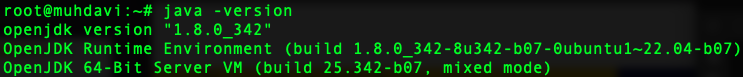
\includegraphics[width=\textwidth]{java-version}
\caption{Versi Java yang Terinstall}
\label{gam:java-version}
\end{figure}

\item Download Apache Hadoop \\
{\tt wget https://dlcdn.apache.org/hadoop/common/hadoop-3.3.4/hadoop-3.3.4.tar.gz}

\item Ekstrak Apache Hadoop \\
{\tt tar -xzvf hadoop-3.3.4.tar.gz }
\begin{itemize}
\item x $\Rightarrow$ ekstrak file arsip.
\item z $\Rightarrow$ filter file arsip melalui gzip.
\item v $\Rightarrow$ menampilkan proses.
\item f $\Rightarrow$ nama file arsip.
\end{itemize}

\item Pindahkan hasil ekstrak ke /usr/local/ \\
{\tt sudo mv hadoop-3.3.4 /usr/local/hadoop}

\item Edit file hadoop-env.sh dengan mengubah variabel JAVA\_HOME\footnote{Pada baris 54, lebih jelasnya lihat Gambar \ref{gam:java-hadoop}} \\
{\tt cd /usr/local/hadoop} \\
{\tt sudo nano etc/hadoop/hadoop-env.sh} \\
\begin{lstlisting}
export JAVA_HOME=/usr/lib/jvm/java-8-openjdk-amd64
\end{lstlisting}

\begin{figure}[!ht]
\centering
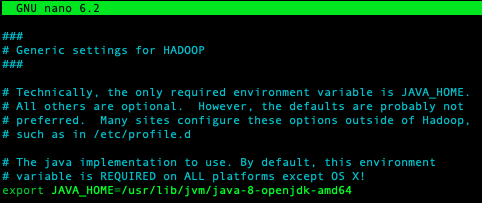
\includegraphics[width=.6\textwidth]{java-hadoop}
\caption{Konfigurasi Java Home}
\label{gam:java-hadoop}
\end{figure}

\item Menambahkan Hadoop Path ke {\tt .bashrc}\footnote{Lebih jelasnya lihat Gambar \ref{gam:hadoop-path}} \\
{\tt sudo nano $\sim$/.bashrc} \\
\begin{lstlisting}
export HADOOP_HOME=/usr/local/hadoop
export HADOOP_CONF_DIR=${HADOOP_HOME}/etc/hadoop
export HADOOP_MAPRED_HOME=${HADOOP_HOME}
export HADOOP_COMMON_HOME=${HADOOP_HOME}
export HADOOP_HDFS_HOME=${HADOOP_HOME}
export YARN_HOME=${HADOOP_HOME}
export PATH=$PATH:/usr/local/hadoop/bin
\end{lstlisting}

{\tt source .bashrc}
\begin{figure}[!ht]
\centering
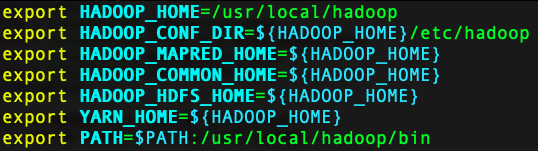
\includegraphics[width=\textwidth]{hadoop-path}
\caption{Konfigurasi Hadoop Path}
\label{gam:hadoop-path}
\end{figure}

\item Verifikasi Hasil Instalasi Hadoop \\
{\tt hadoop version} \\
Jika instalasi hadoop sudah berhasil, maka ketika mengecek versi hadoop akan muncul seperti yang diperlihatkan pada Gambar \ref{gam:hadoop-version}.
\begin{figure}[!ht]
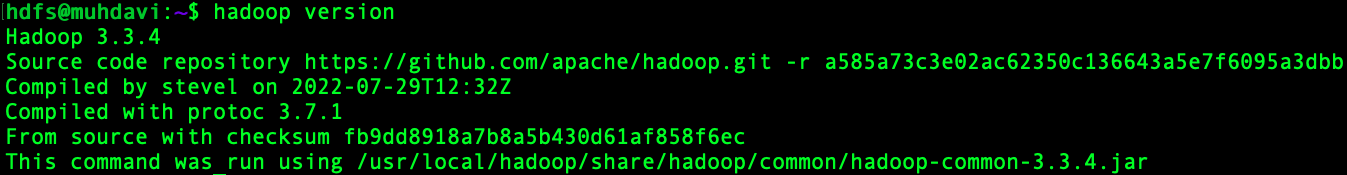
\includegraphics[width=\textwidth]{hadoop-version}
\caption{Versi Hadoop yang Terinstall}
\label{gam:hadoop-version}
\end{figure}
\end{enumerate}
 
\hrulefill

%%%%%%%%%%%%%%%%%%%%%%%%%%%%%%%%%%%%%%%%%%%%%%%%%%%%%%%%
\clearpage
\newday{\#3 - 22 September 2022}
\textit{N.B.: Setiap mahasiswa membuat laporan hasil praktik sesuai dengan format yang telah ditentukan. Template laporan dapat di download pada alamat \url{https://github.com/muhdavi/laporan-practice-big-data}.}

\newthought{Konfigurasi Apache Hadoop}

Setelah selesai meng-install Hadoop, kita perlu konfigurasi beberapa file Hadoop agar memudahkan kita dalam memonitoring ekosistem Hadoop yang telah diinstall.

\begin{enumerate}
\item Konfigurasi File Hadoop \\
File-file konfigurasi hadoop berada pada folder {\tt hadoop/etc/hadoop} seperti yang diperlihatkan pada Gambar \ref{gam:file-hadoop}.
{\tt cd /usr/local/hadoop/etc/hadoop} \\
{\tt ls}
\begin{figure}[!ht]
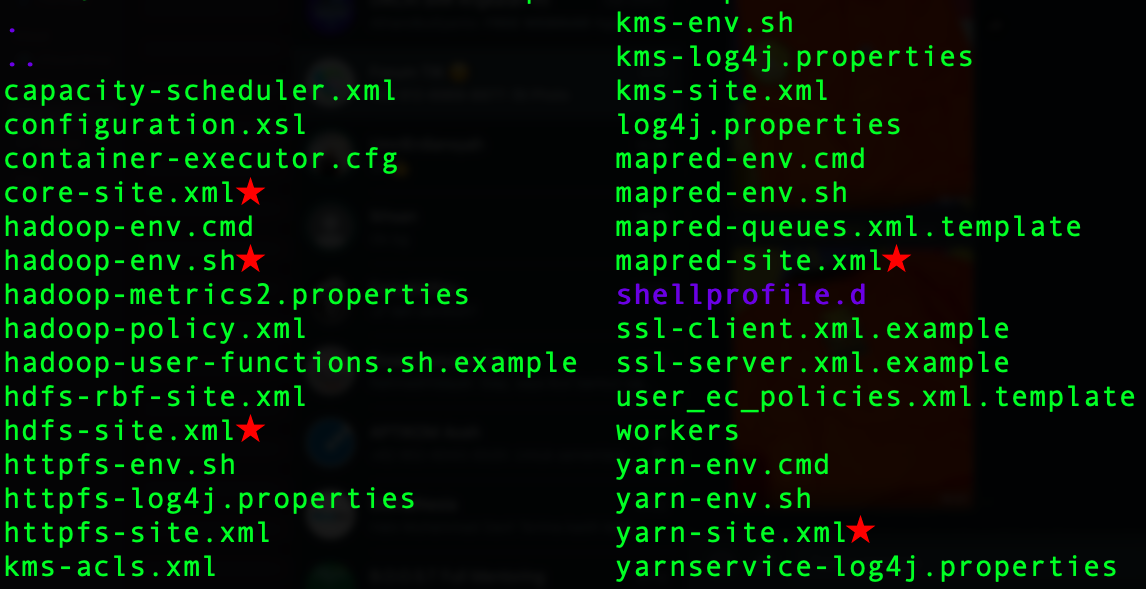
\includegraphics[width=\textwidth]{file-hadoop}
\caption{File Konfigurasi Hadoop}
\label{gam:file-hadoop}
\end{figure}

Beberapa file yang perlu dikonfigurasi adalah sebebai berikut:
\begin{itemize}

\item core-site.xml
\begin{lstlisting}
<property>
	<name>fs.default.name</name>
	<value>hdfs://localhost:9000</value>
</property>
\end{lstlisting}
\begin{figure}[!ht]
\centering
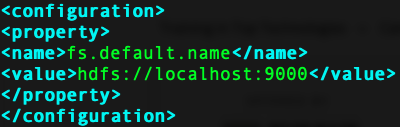
\includegraphics[width=.8\textwidth]{site-core}
\caption{Konfigurasi Core Site}
\label{gam:site-yarn}
\end{figure}

\item hdfs-site.xml
\begin{lstlisting}
<property>
	<name>dfs.replication</name>
	<value>1</value>
</property>
<property>
	<name>dfs.permission</name>
	<value>false</value>
</property>
\end{lstlisting}
\begin{figure}[!ht]
\centering
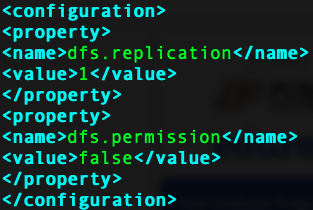
\includegraphics[width=.7\textwidth]{site-hdfs}
\caption{Konfigurasi HDFS Site}
\label{gam:site-yarn}
\end{figure}

\item mapred-site.xml
\begin{lstlisting}
<property>
	<name>mapreduce.framework.name</name>
	<value>yarn</value>
</property>
\end{lstlisting}
\begin{figure}[!ht]
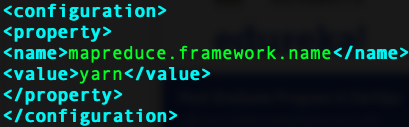
\includegraphics[width=\textwidth]{site-mapred}
\caption{Konfigurasi Mapred Site}
\label{gam:site-yarn}
\end{figure}

\item yarn-site.xml
\begin{lstlisting}
<property>
	<name>yarn.nodemanager.aux-services</name>
	<value>mapreduce_shuffle</value>
</property>
<property>
	<name>yarn.nodemanager.auxservices.mapreduce.shuffle.class</name>
	<value>org.apache.hadoop.mapred.ShuffleHandler</value>
</property>
\end{lstlisting}
\begin{figure}[!ht]
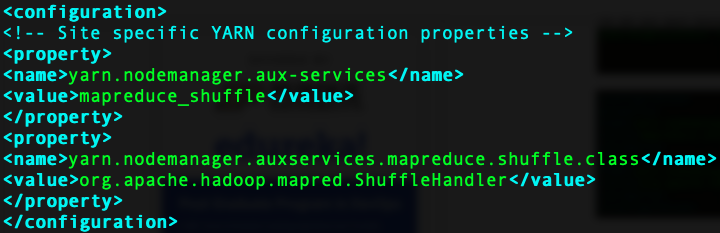
\includegraphics[width=\textwidth]{site-yarn}
\caption{Konfigurasi Yarn Site}
\label{gam:site-yarn}
\end{figure}
\end{itemize}

\item Jalankan Perintah Format Filesystem \\
{\tt hdfs namenode -format}
\begin{figure}[!ht]
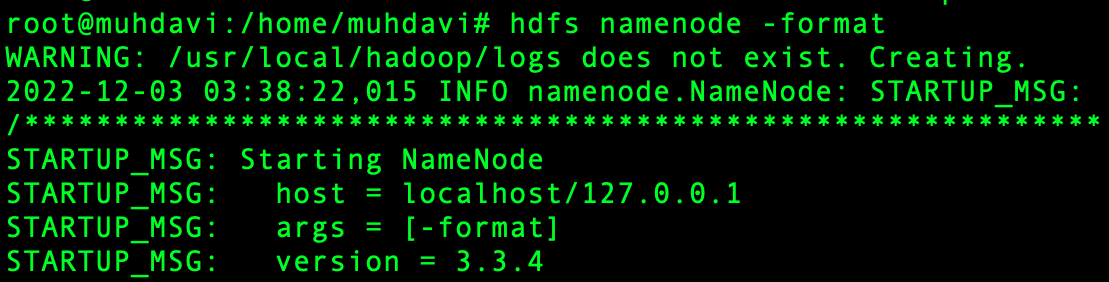
\includegraphics[width=\textwidth]{format-filesystem}
\caption{Format Filesystem}
\label{gam:format-filesystem}
\end{figure}

\item Jalankan NameNode Daemon dan DataNode Daemon \\
{\tt sbin/start-dfs.sh} \\
NameNode dapat diakses melalui \url{http://localhost:9870} dan akan tampil halaman web seperti yang diperlihatkan pada Gambar \ref{gam:namenode}.
\begin{figure}[!ht]
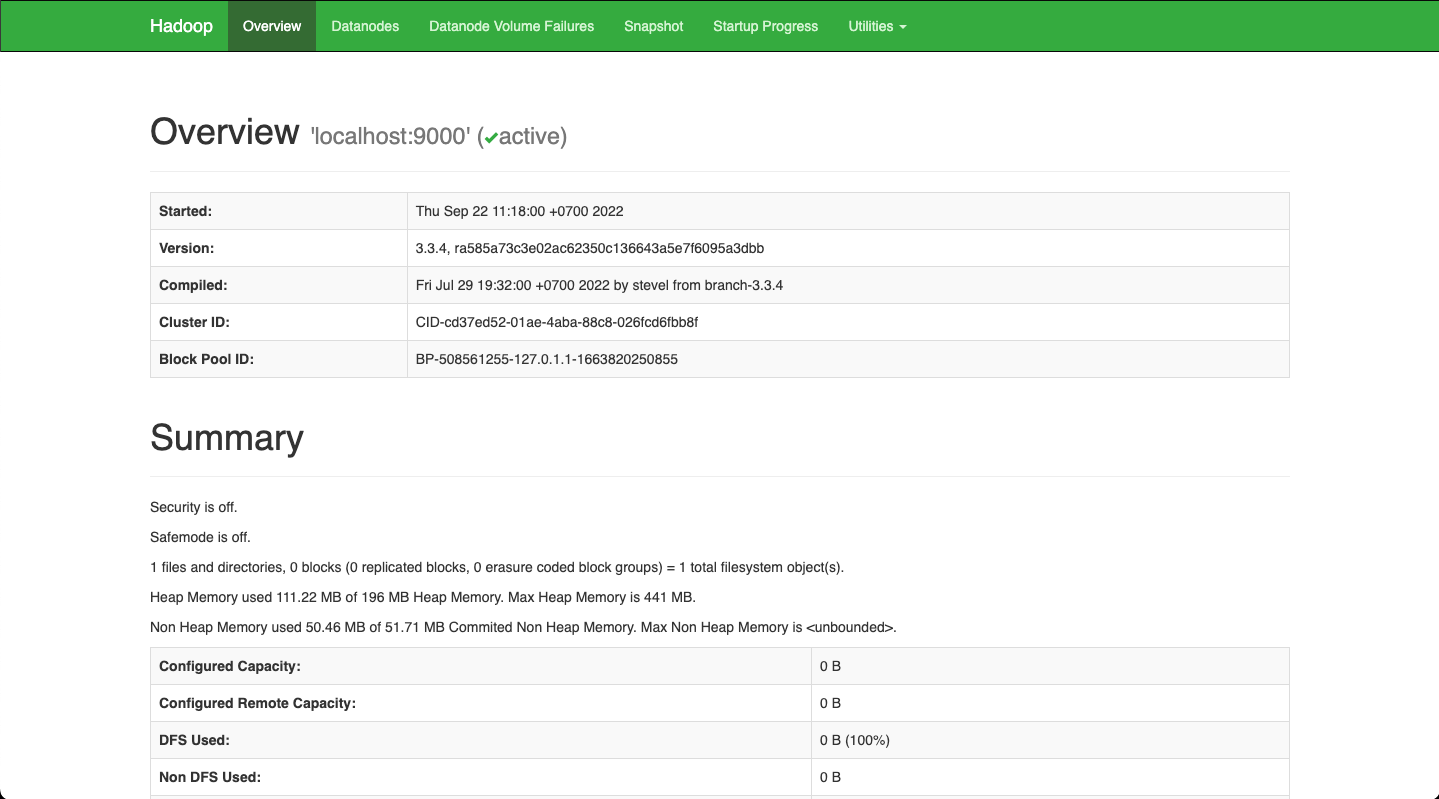
\includegraphics[width=\textwidth]{namenode}
\caption{Namemnode Hadoop}
\label{gam:namenode}
\end{figure}

\item Jalankan ResourceManager Daemon and NodeManager Daemon \\
{\tt sbin/start-yarn.sh} \\
ResourceManager dapat diakses melalui \url{http://localhost:8088} dan akan tampil halaman web serperti pada Gambar \ref{gam:namenode}.
\begin{figure}[!ht]
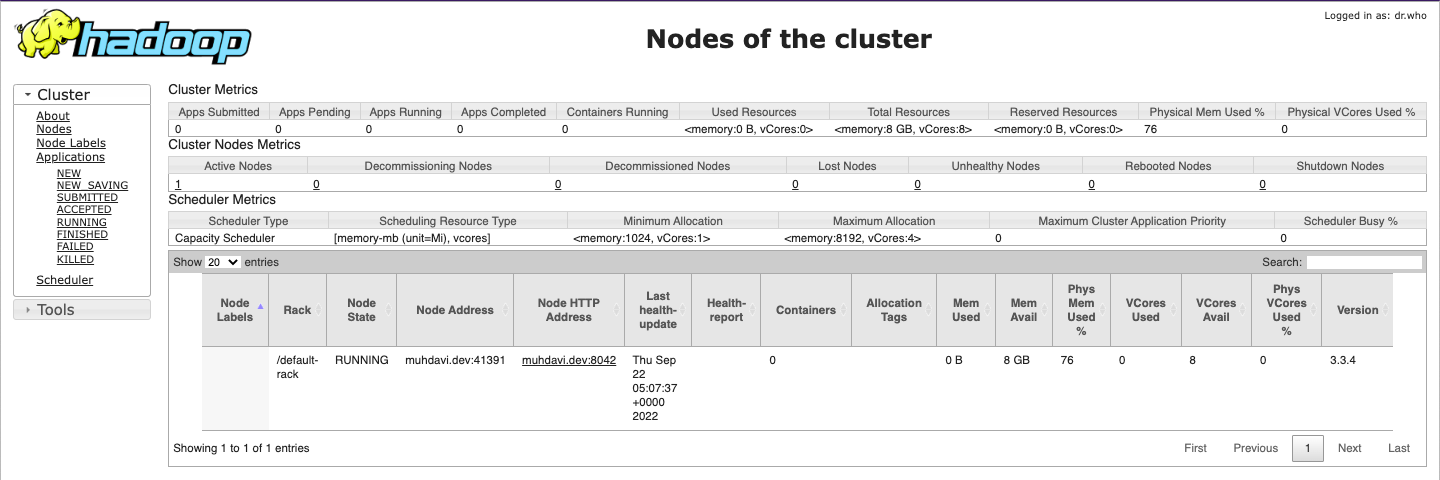
\includegraphics[width=\textwidth]{resourcemanager}
\caption{Resource Manager Hadoop}
\label{gam:resourcemanager}
\end{figure}
\end{enumerate}

Proses analisis big data sebaiknya menggunakan komputer dengan spesifikasi yang tinggi atau \textit{High Performance Computer (HPC)}. Namun jika tidak memiliki HPC cara lain adalah dengan menggabungkan beberapa komputer untuk melakukan proses analisis yang dikenal dengan nama \textit{Parallel Computing}. Paga Gambar \ref{gam:resourcemanager} terlihat bahwa ada 1 Node yang aktif, artinya jika diterapkan \textit{Parallel Computing} maka akan ada beberapa Node yang terhubung/aktif pada tampilan tersebut.

\hrulefill

%%%%%%%%%%%%%%%%%%%%%%%%%%%%%%%%%%%%%%%%%%%%%%%%%%%%%%%%
\clearpage
\newday{\#4 - 24 November 2022 menggantikan 29 September 2022}

\newthought{Instalasi dan Konfigurasi GIT dan GitHub}

Pada pertemuan kali ini kita belajar install GIT dan konfigurasi GIT dengan GitHub agar dapat menjalankan perintah-perintah GIT melalui lokal dan menyimpan hasil kerjaan kita ke GitHub. Karena pada pertemuan pertama telah membuat akun GitHub, maka pada pertemuan kali ini asumsinya semua sudah memiliki akun GitHub. Setelah itu ikuti beberapa langkah berikut untuk praktikum kali ini.

\begin{enumerate}
\item Install Git \\
Pertema download program Git melalui link ini (\url{https://git-scm.com/download}) sesuai dengan sistem operasi yang digunakan. Bagi pengguna Windows jika proses download sudah selesai, lanjut proses instalasi seperti program windows pada umumnya (Next, Next, Next, sampai selesai).

\item \textit{Generate} SSH-Key \\
Jika instalasi sudah selesai, coba buka Git Bash, maka akan muncul program baru yang mirip dengan Terminal atau Command Prompt (CMD) kita sebut Git Bash. Kemudian jalankan perintah berikut untuk \textit{generate ssh-key}.

{\tt ssh-keygen -t ed25519 -C "email@akun.github"} \\

Ganti {\tt email@akun.github} dengan email yang terdaftar pada akun GitHub. Selanjutnya jika muncul beberapa pertanyaan seperti berikut ini tekan [enter].

{\tt > Enter a file in which to save the key (/Users/YOU/.ssh/id\_ed25519:} \\
{\tt > Enter passphrase (empty for no passphrase):} \\
{\tt > Enter same passphrase again:}

Jika proses diatas berhasil maka terbentuk folder baru dengan nama {\tt .ssh}. Didalam folder tersebut terdapat \textit{private key} dan \textit{public key}. Bukan file \textit{public key} (id\_ed25519.pub) dan \textit{copy} isi dari file tersebut.

\item Menambahkan SSH-Key ke Akun GitHub \\
Untuk menambahkan SSH-Key ke akun GitHub pertama login terlebih dahulu. Setelah berhasil login klik pada gambar profil sehingga tampil menu dropdown seperti pada Gambar \ref{gam:langkah-ssh} nomor 1. Selanjutnya pilih menu \textbf{Setting} sepertin yang ditunukan pada nomor 2. Setelah memilih menu \textbf{Setting} maka muncul halaman setting dengan menu di sidebar sebelah kiri. Pada menu sebelah kiri pilih menu \textbf{SSH and GPG keys} seperti pada nomor 3. Kemudian klik tombol \textbf{New SSH key} maka akan muncul form menambahkan SSH seperti yang diperlihatkan pada Gambar \ref{gam:form-ssh}.

\begin{figure}[!ht]
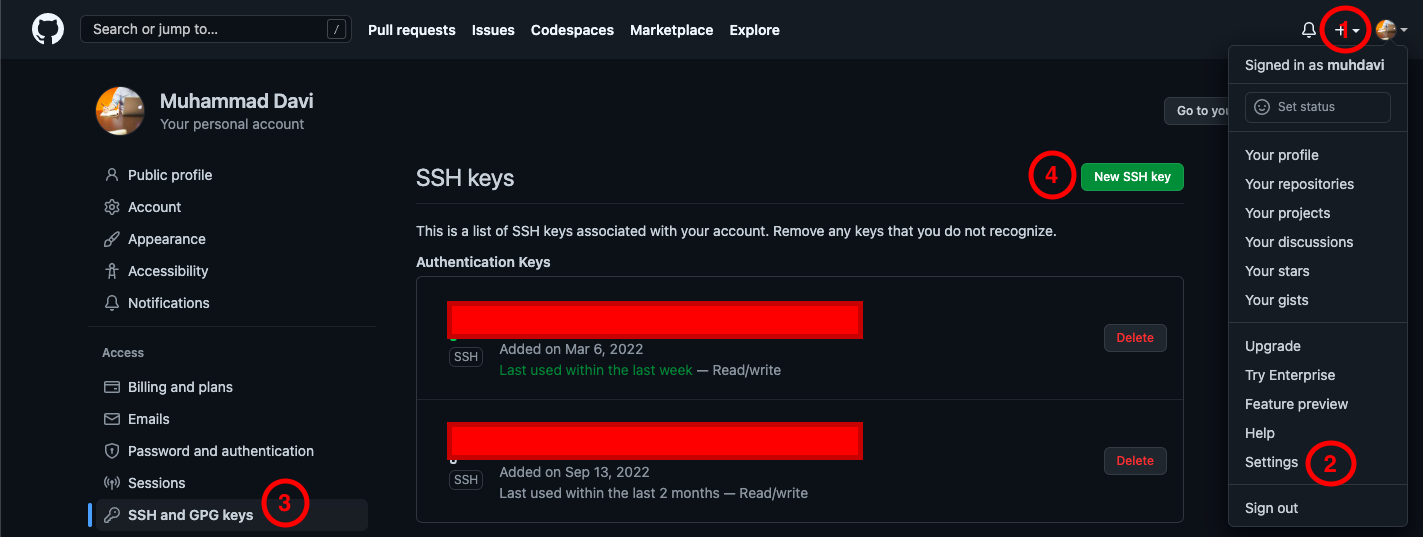
\includegraphics[width=\textwidth]{gtihub-1}
\caption{Lankah-langkah Menambah SSH-Key di GitHub}
\label{gam:langkah-ssh}
\end{figure}

Kode SSH-Key yang telah di-\textit{copy} pada langkah sebelumnya \textit{paste}-kan kode tersebut pada isian \textbf{Key} dan beri judul SSH-Key pada isian \textbf{Title}. Setelah semua diisi klik tombol \textbf{Add SSH key} untuk menyimpan SSH-Key baru tersebut.

\begin{figure}[!ht]
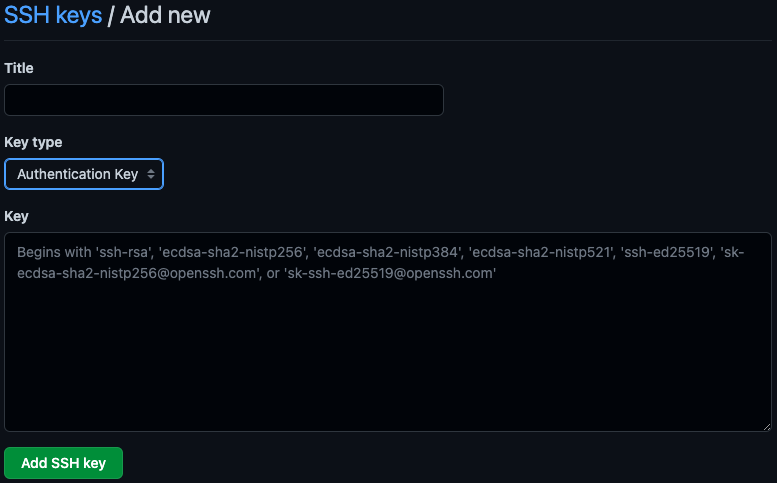
\includegraphics[width=\textwidth]{github-2}
\caption{Form Penambahan SSH-Key di GitHub}
\label{gam:form-ssh}
\end{figure}

Untuk menguji bahwa penambahan SSH-Key telah berhasil coba lakukan {\tt git push} untuk repositori laporan practice big data dari akun masing-masing. Untuk lebih jelasnya tentang GIT dapat membaca catatan pada link berikut \url{https://muhdavi.github.io/learn-git/}.
\end{enumerate}

\begin{figure}[!ht]
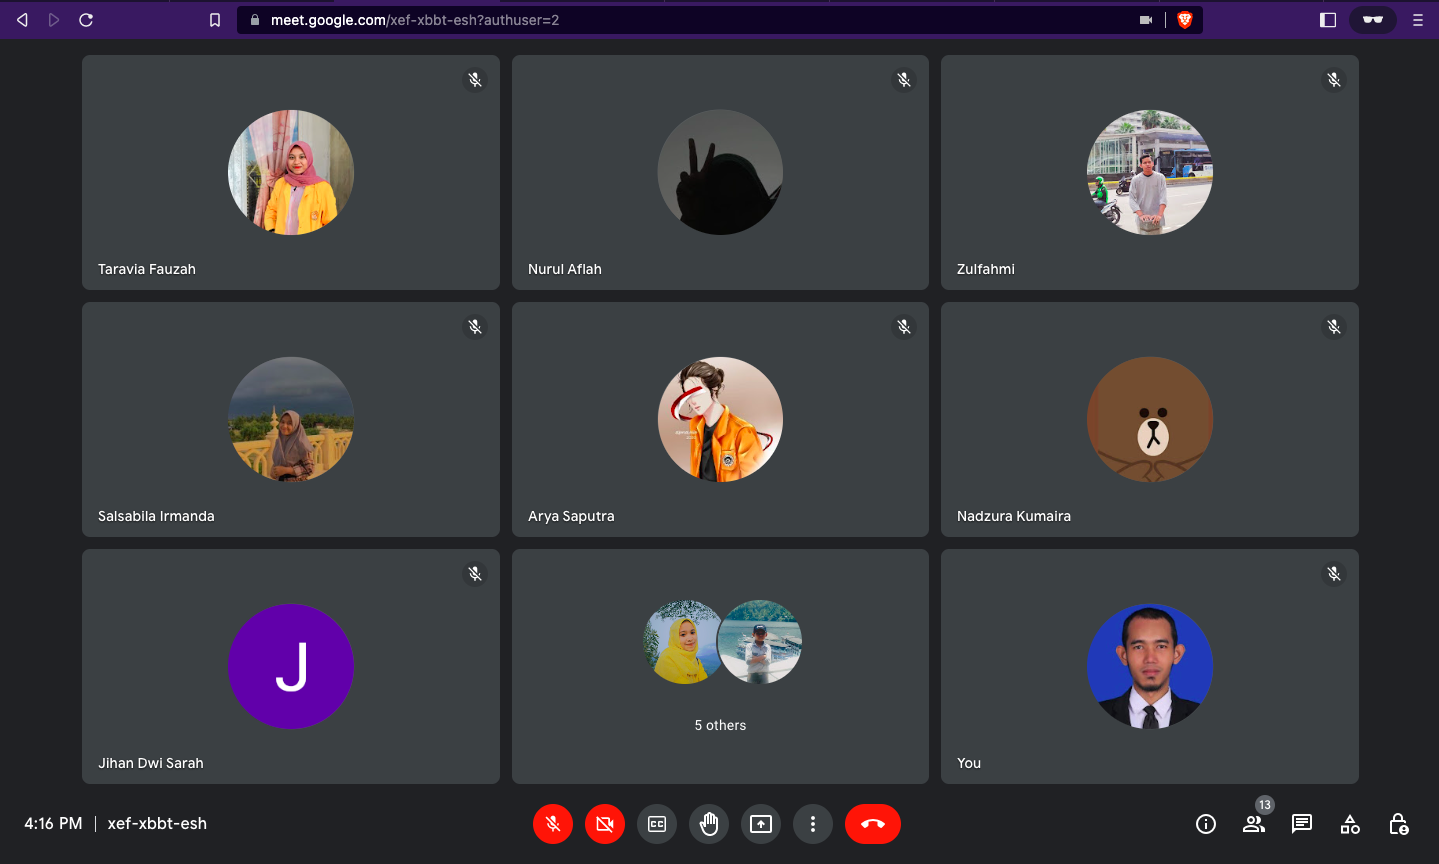
\includegraphics[width=.95\textwidth]{24-11-2022}
\caption{Perkuliahan Daring via GMeet 24-11-2022}
\label{gam:form-ssh}
\end{figure}

%%%%%%%%%%%%%%%%%%%%%%%%%%%%%%%%%%%%%%%%%%%%%%%%%%%%%%%%
\clearpage
\newday{\#5 - 25 November 2022 menggantikan 6 Oktober 2022}

\newthought{Instalasi dan Konfigurasi GIT dan GitHub - Lanjutan}

Mahasiswa yang sudah berhasil konfigurasi Git dengan GitHub dan melalkukan {\tt Pull Request}:
\begin{multicols}{2}
\begin{enumerate}
\item Rizki Ilhami
\item Rauzatinur Syah $\star$
\item Taravia Fauzah
\item Resha Russita $\star$
\item Nurani Harum Fardaniah $\star$
\item Adinda Awaliah $\star$
\item Salsabila Irmanda $\star$
\item M. Ikhsan
\item Jihan Dwi Sarah $\star$
\item Cut Opy Mandalisa $\star$
\item Zulfahmi
\item Muhammad Munawir
\item Nuraula Tafiza
\item Muhammad Ikrammullah
\item Nadzura Kumaira
\end{enumerate}
\end{multicols}

\noindent
Berikut beberapa mahasiswa yang belum melakukan {\tt Pull Request}:
\begin{multicols}{2}
\begin{enumerate}
\item \textcolor{purple}{Adjie Yusmunandar}
\item Arya Saputra
\item Faiza Yuwafiqi
\item Nurul Aflah
\item \textcolor{red}{Siti Hajar Al Zahra}
\item Syarfani Akbar
\end{enumerate}
\end{multicols}

\begin{figure}[!ht]
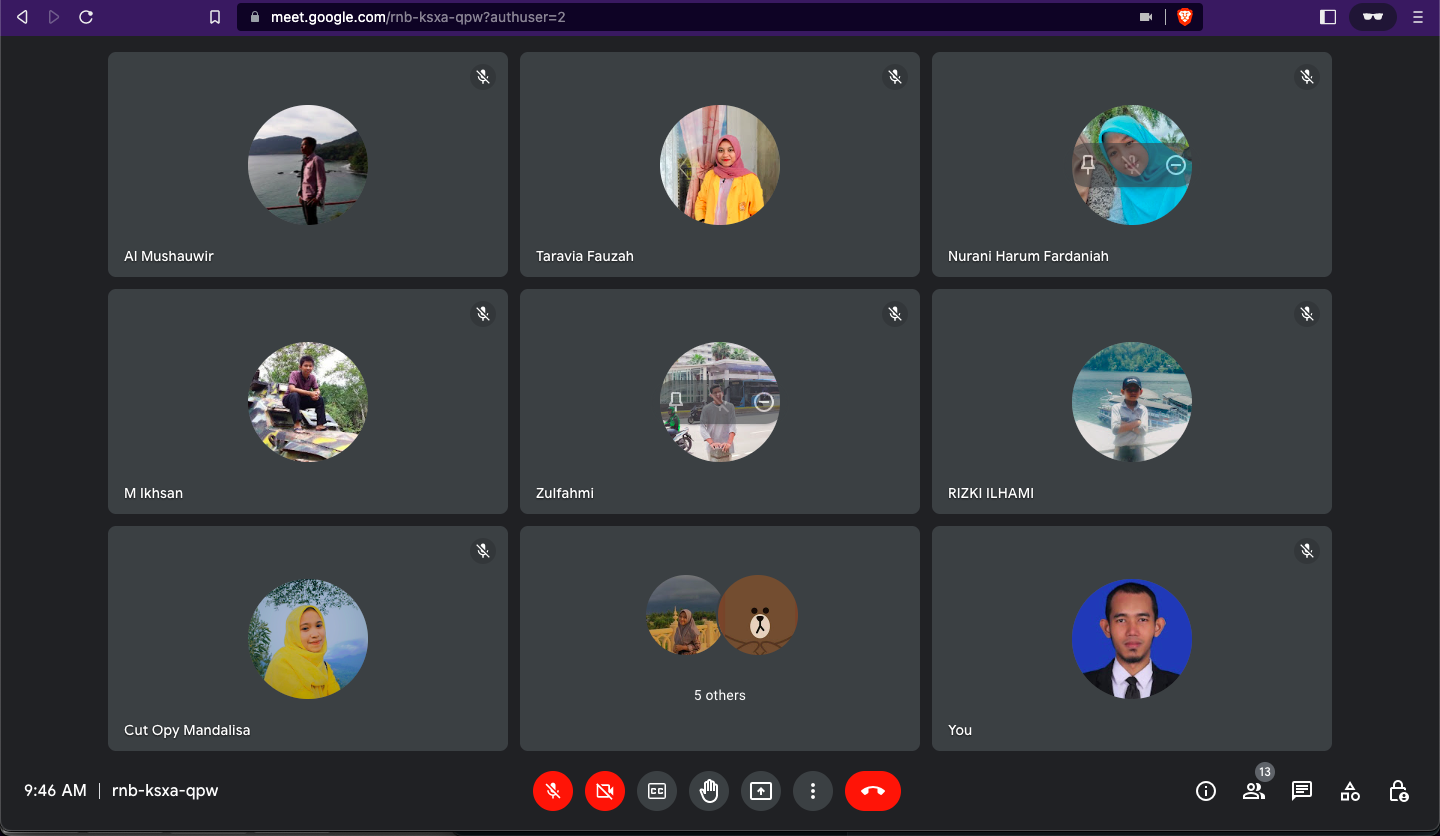
\includegraphics[width=\textwidth]{25-11-2022}
\caption{Perkuliahan Daring via GMeet 25-11-2022}
\label{gam:form-ssh}
\end{figure}

%%%%%%%%%%%%%%%%%%%%%%%%%%%%%%%%%%%%%%%%%%%%%%%%%%%%%%%%
\clearpage
\newday{\#6 - 1 Desember 2022 menggantikan 13 Oktober 2022}

\newthought{Instalasi Apache Pig}

\begin{enumerate}
\item Download Apache Pig  \\
Apache Pig dapat didownload dari link ini \url{https://downloads.apache.org/pig/pig-0.17.0/pig-0.17.0.tar.gz} menggunakan {\tt wget} sehingga akan ada file baru dengan nama {\tt pig-0.17.0.tar.gz}

{\tt wget https://downloads.apache.org/pig/pig-0.17.0/pig-0.17.0.tar.gz}

\item Ekstrak Apache Pig \\
Ekstrak hasil download tadi dengan perintah {\tt tar}

{\tt tar -xzvf pig-0.17.0.tar.gz}

\item Pindahkan Hasil Ekstraksi \\
Pindahkan hasil ekstraksi ke {\tt /usr/local/} dengan perintah {\tt mv}

{\tt sudo mv pig-0.17.0 /usr/local/pig}

\item Tambahkan Path Apache Pig ke {\tt .bashrc} \\
Untuk menambahkan path apache pig ke {\tt .bashrc} gunakan perintah nano

{\tt sudo nano $\sim$/.bashrc}

\begin{lstlisting}
#Apache Pig location
export PIG_INSTALL=/usr/local/pig
export PATH=$PATH:/usr/local/pig/bin
\end{lstlisting}

Kemdudian jalankan perintah {\tt source} agar konfigurasi yang telah ditambahkan ke {\tt .bashrc} dapat dikenali oleh sistem dan memastikan konfigurasi tersebut sudah benar.

{\tt source .bashrc}

\item Verifikasi Apache Pig \\
Untuk memverifikasi bahwa instalasi telah berhasil, coba cek versi Apache Pig dengan perintah berikut:

{\tt pig -version}
\end{enumerate}

%%%%%%%%%%%%%%%%%%%%%%%%%%%%%%%%%%%%%%%%%%%%%%%%%%%%%%%%
\clearpage
\newday{\#7 - 2 Desember 2022 menggantikan 20 Oktober 2022}

\newthought{Instalasi Apache Hive}

\begin{enumerate}
\item Download Apaceh Hive \\
Download Apache Hive melalui link ini \url{https://downloads.apache.org/hive/stable-2/apache-hive-2.3.9-bin.tar.gz} dengan menggunakan perintah {\tt wget} seperti berikut:

{\tt wget https://downloads.apache.org/hive/stable-2/apache-hive-2.3.9-bin.tar.gz}

\item Ekstrak Apache Hive \\
Ekstrak file yang telah didownload dengna perintah berikut:

{\tt tar -zxvf apache-hive-2.3.9-bin.tar.gz}

\item Pindahkan Hasil Ekstraksi \\
Pindahkan hasil ekstraksi ke {\tt /usr/local/} dengan perintah {\tt mv}

{\tt sudo mv apache-hive-2.3.9-bin /usr/local/hive}

\item Tambahkan Path Apaceh Hive ke {\tt .bashrc} \\
Untuk menambahkan path apache hive ke {\tt .bashrc} gunakan perintah nano
seperti berikut:

{\tt sudo nano $\sim$/.bashrc}

\begin{lstlisting}
#Apache Hive location
export HIVE_HOME=/usr/local/hive
export PATH=$PATH:/usr/local/hive/bin
\end{lstlisting}

\item Konfigurasi {\tt core-site.xml} \\
Buka file {\tt core-site.xml} yang berada di {\tt /usr/local/hadoop/etc/hadoop} dan update seperti pada kode berikut:

\begin{lstlisting}
<configuration>
	<property>
		<name>fs.default.name</name>
		<value>hdfs://localhost:9000</value>
	</property>
	<property>
		<name>hadoop.tmp.dir</name>
		<value>/home/muhdavi/hadoop/tmp</value>
	</property>
	<property>
		<name>hadoop.proxyuser.dataflair.groups</name>
		<value>*</value>
	</property>
	<property>
		<name>hadoop.proxyuser.dataflair.hosts</name>
		<value>*</value>
	</property>
	<property>
		<name>hadoop.proxyuser.server.hosts</name>
		<value>*</value>
	</property>
	<property>
		<name>hadoop.proxyuser.server.groups</name>
		<value>*</value>
	</property>
</configuration>
\end{lstlisting}

\item Membuat directory di HDPS \\
Buatlah beberapa directory berikut di HDPS dengan perintah sebagai berikut:

{\tt \$hadoop fs -mkdir /tmp} \\
{\tt \$hadoop fs -mkdir /user} \\
{\tt \$hadoop fs -mkdir /user/hive} \\
{\tt \$hadoop fs -mkdir /user/hive/warehouse}

\item Memberikan Hak Akses \\
Memberikan hak akses (\textit{permission}) pada folder berikut:

{\tt \$hadoop fs -chmod g+w /tmp} \\
{\tt \$hadoop fs -chmod g+w /user/hive/warehouse}

\item Inisialisasi Hive Database

{\tt \$bin/schematool -dbType derby -initSchema}

\item Jalankan Hive

{\tt \$bin/hiveserver2}

\item Verifikasi Hive \\
Buka terminal baru dan coba konek ke Hive dengan perintah berikut:

{\tt \$bin/beeline -n bigdata -u jdbc:hive2://localhost:10000}

\end{enumerate}

%%%%%%%%%%%%%%%%%%%%%%%%%%%%%%%%%%%%%%%%%%%%%%%%%%%%%%%%
\clearpage
\newday{\#8 - 8 Desember 2022 menggantikan 3 November 2022}

\newthought{Analisis Data Youtube}

\begin{enumerate}
\item Download Dataset \\
Dataset dapat didownload dengan perintah berikut.

{\tt wget http://netsg.cs.sfu.ca/youtubedata/0222.zip}

\item Kode Apache Pig \\
Tulis kode Apache Pig berikut menggunakan IDE.

\begin{lstlisting}
infiles = load '/hdfs/bhavesh/Youtube_POC/Youtube/0222/{0,1,2,3,4}.txt' using PigStorage('\t') as 
(videoid:chararray,uploader:chararray,age:int,category:chararray,length:int,views:int,rate:int,rating:int,comments:int,related_id:chararray);
files = FILTER infiles BY category is not null;
grpn_for_catagories = group files by category;
cnt_for_catagories = foreach grpn_for_catagories generate group, COUNT(files.videoid) as counting;
sorted_for_catagories_desc = order cnt_for_catagories by counting desc;
top5_for_catagories = limit sorted_for_catagories_desc 5;
STORE top5_for_catagories INTO  '/hdfs/bhavesh/Youtube_POC/Top5Catagories' using PigStorage(',');
order_rated_video = order files by rating desc;
top10_rated_video = limit order_rated_video 10;
final_top10_rated_video = foreach top10_rated_video generate $0,$3,$7;
STORE final_top10_rated_video INTO '/hdfs/bhavesh/Youtube_POC/Top10Rated' using PigStorage(',');
order_viewed_video = order files by views desc;
top10_viewed_video = limit order_viewed_video 10;
final_top10_viewed_video = foreach top10_viewed_video generate $0,$3,$5;
STORE final_top10_viewed_video INTO '/hdfs/bhavesh/Youtube_POC/Top10Viewed' using PigStorage(',');
top10_rated_catagories = foreach grpn_for_catagories{
                           sorted = order files by rating desc;
                           top10 = limit sorted 10;
                           generate flatten(top10);
};
top10_rated_by_catagories = foreach top10_rated_catagories generate $0,$3,$7;
STORE top10_rated_by_catagories INTO '/hdfs/bhavesh/Youtube_POC/Top10RatedByCatagories' using PigStorage(',');
top10_viewed_catagories = foreach grpn_for_catagories{
                           sorted = order files by views desc;
                           top10 = limit sorted 10;
                           generate flatten(top10);
};
top10_viewed_by_catagories = foreach top10_viewed_catagories generate $0,$3,$5;
STORE top10_viewed_by_catagories INTO '/hdfs/bhavesh/Youtube_POC/Top10ViewedByCatagories' using PigStorage(',');
\end{lstlisting}

\item Kode Shell Script

\begin{lstlisting}
sudo rm -rf /var/lib/hive/metastore/metastore_db/*.lck
rm /home/mrinmoy/Downloads/POC/YoutubePOC/Top5Catagories.csv
rm /home/mrinmoy/Downloads/POC/YoutubePOC/Top10Rated.csv
rm /home/mrinmoy/Downloads/POC/YoutubePOC/Top10RatedByCatagories.csv
rm /home/mrinmoy/Downloads/POC/YoutubePOC/Top10Viewed.csv
rm /home/mrinmoy/Downloads/POC/YoutubePOC/Top10ViewedByCatagories.csv
hadoop fs -rmr /hdfs/bhavesh/Youtube_POC/Top5Catagories
hadoop fs -rmr /hdfs/bhavesh/Youtube_POC/Top10Rated
hadoop fs -rmr /hdfs/bhavesh/Youtube_POC/Top10RatedByCatagories
hadoop fs -rmr /hdfs/bhavesh/Youtube_POC/Top10Viewed
hadoop fs -rmr /hdfs/bhavesh/Youtube_POC/Top10ViewedByCatagories
pig /home/bhavesh/Youtube_POC/Youtube/0222/Youtube_data_analysis.pig
hadoop fs -get /hdfs/bhavesh/Youtube_POC/Top5Catagories/part-r-00000               /home/mrinmoy/Downloads/POC/YoutubePOC/Top5Catagories.csv
hadoop fs -get /hdfs/bhavesh/Youtube_POC/Top10Rated/part-r-00000                   /home/mrinmoy/Downloads/POC/YoutubePOC/Top10Rated.csv
hadoop fs -get /hdfs/bhavesh/Youtube_POC/Top10RatedByCatagories/part-r-00000       /home/mrinmoy/Downloads/POC/YoutubePOC/Top10RatedByCatagories.csv
hadoop fs -get /hdfs/bhavesh/Youtube_POC/Top10Viewed/part-r-00000                  /home/mrinmoy/Downloads/POC/YoutubePOC/Top10Viewed.csv
hadoop fs -get /hdfs/bhavesh/Youtube_POC/Top10ViewedByCatagories/part-r-00000      /home/mrinmoy/Downloads/POC/YoutubePOC/Top10ViewedByCatagories.csv
hive -e 'drop table if exists Top5CatagoriesTable';
hive -e 'drop table if exists Top10RatedTable';
hive -e 'drop table if exists Top10RatedByCatagoriesTable';
hive -e 'drop table if exists Top10ViewedTable';
hive -e 'drop table if exists Top10ViewedByCatagoriesTable';
hive -e "create external table Top5CatagoriesTable(Top5Catagory string, VideoCount int) row format delimited fields terminated by',' lines terminated by '\n' stored as textfile location '/hdfs/bhavesh/Youtube_POC/hive/Top5Catagories'";
hive -e "create external table Top10RatedTable(Videoid string,Catagory string,Rating int) row format delimited fields terminated by',' lines terminated by '\n' stored as textfile location '/hdfs/bhavesh/Youtube_POC/hive/Top10RatedTable'";
hive -e "create external table Top10RatedByCatagoriesTable(Videoid string,Catagory string,Rating int) row format delimited fields terminated by',' lines terminated by '\n' stored as textfile location '/hdfs/bhavesh/Youtube_POC/hive/Top10RatedByCatagoriesTable'";
hive -e "create external table Top10ViewedTable(Videoid string,Catagory string,Viewed_count int) row format delimited fields terminated by',' lines terminated by '\n' stored as textfile location '/hdfs/bhavesh/Youtube_POC/hive/Top10ViewedTable'";
hive -e "create external table Top10ViewedByCatagoriesTable(Videoid string,Catagory string,Viewed_count int) row format delimited fields terminated by',' lines terminated by '\n' stored as textfile location '/hdfs/bhavesh/Youtube_POC/hive/Top10ViewedByCatagoriesTable'";
hive -e "load data inpath '/hdfs/bhavesh/Youtube_POC/Top5Catagories/part-r-00000' overwrite into table Top5CatagoriesTable";
hive -e "load data inpath '/hdfs/bhavesh/Youtube_POC/Top10Rated/part-r-00000' overwrite into table Top10RatedTable";
hive -e "load data inpath '/hdfs/bhavesh/Youtube_POC/Top10RatedByCatagories/part-r-00000' overwrite into table Top10RatedByCatagoriesTable";
hive -e "load data inpath '/hdfs/bhavesh/Youtube_POC/Top10Viewed/part-r-00000' overwrite into table Top10ViewedTable";
hive -e "load data inpath '/hdfs/bhavesh/Youtube_POC/Top10ViewedByCatagories/part-r-00000' overwrite into table Top10ViewedByCatagoriesTable";
\end{lstlisting}

\item Jalankan Shell Script
\item Cek Hasil CSV
\item Cek Hasil Hive
\end{enumerate}

%%%%%%%%%%%%%%%%%%%%%%%%%%%%%%%%%%%%%%%%%%%%%%%%%%%%%%%%

\newthought{\textbf{Adinda Awaliah - 2020903430004 - TRKJ 3B}}

\newday{\textbf{15 september 2022}}
\begin{enumerate}
\item Kendala dan Solusi
% jelaskan kendala dan penyebab yang dialami saat mengikuti praktikum serta solusi atau langkah-langkah yang telah dilakukan
\newline praktikum instalasi apache hadoop tidak ada kendala.

\item Kesimpulan
% berikan kesimpulan dari praktikum yang telah dikerjkan
\newline berhasil melakukan instalasi.

\begin{figure}
\setlength{\belowcaptionskip}{-10pt}
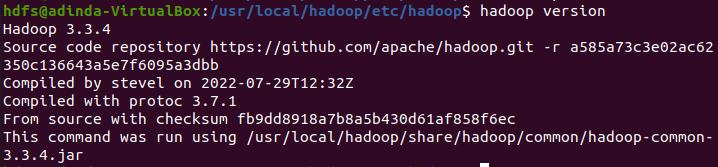
\includegraphics[width=\textwidth]{AdindaAwaliah/hasil instalasi apache hadoop}
\caption{Versi Java yang Terinstall}
\label{gam:hasil instalasi apache hadoop}
\end{figure}

\end{enumerate}

\newday{\textbf{1 desember 2022}}
\begin{enumerate}
\item Kendala dan Solusi
% jelaskan kendala dan penyebab yang dialami saat mengikuti praktikum serta solusi atau langkah-langkah yang telah dilakukan

\item Kesimpulan
% berikan kesimpulan dari praktikum yang telah dikerjkan

\end{enumerate}

\newday{\textbf{02 desember 2022}}
\begin{enumerate}
\item Kendala dan Solusi
% jelaskan kendala dan penyebab yang dialami saat mengikuti praktikum serta solusi atau langkah-langkah yang telah dilakukan

\item Kesimpulan
% berikan kesimpulan dari praktikum yang telah dikerjkan

\end{enumerate}

\newday{\textbf{08 desember 2022}}
\begin{enumerate}
\item Kendala dan Solusi
% jelaskan kendala dan penyebab yang dialami saat mengikuti praktikum serta solusi atau langkah-langkah yang telah dilakukan

\item Kesimpulan
% berikan kesimpulan dari praktikum yang telah dikerjkan

\end{enumerate}

\newday{\textbf{09 desember 2022}}
\begin{enumerate}
\item Kendala dan Solusi
% jelaskan kendala dan penyebab yang dialami saat mengikuti praktikum serta solusi atau langkah-langkah yang telah dilakukan

\item Kesimpulan
% berikan kesimpulan dari praktikum yang telah dikerjkan

\end{enumerate}

\newday{\textbf{15 desember 2022}}
\begin{enumerate}
\item Kendala dan Solusi
% jelaskan kendala dan penyebab yang dialami saat mengikuti praktikum serta solusi atau langkah-langkah yang telah dilakukan

\item Kesimpulan
% berikan kesimpulan dari praktikum yang telah dikerjkan

\end{enumerate}

\newday{\textbf{16 desember 2022}}
\begin{enumerate}
\item Kendala dan Solusi
% jelaskan kendala dan penyebab yang dialami saat mengikuti praktikum serta solusi atau langkah-langkah yang telah dilakukan

\item Kesimpulan
% berikan kesimpulan dari praktikum yang telah dikerjkan

\end{enumerate}

\newday{\textbf{22 desember 2022}}
\begin{enumerate}
\item Kendala dan Solusi
% jelaskan kendala dan penyebab yang dialami saat mengikuti praktikum serta solusi atau langkah-langkah yang telah dilakukan

\item Kesimpulan
% berikan kesimpulan dari praktikum yang telah dikerjkan

\end{enumerate}

\newday{\textbf{23 desember 2022}}
\begin{enumerate}
\item Kendala dan Solusi
% jelaskan kendala dan penyebab yang dialami saat mengikuti praktikum serta solusi atau langkah-langkah yang telah dilakukan

\item Kesimpulan
% berikan kesimpulan dari praktikum yang telah dikerjkan

\end{enumerate}

\newthought{\textbf{Adjie Yusmunandar - 2020903430005 - TRKJ 3B}}

\newday{\textbf{22 September 2022}}
\begin{enumerate}
\item Kendala dan Solusi
% jelaskan kendala dan penyebab yang dialami saat mengikuti praktikum serta solusi atau langkah-langkah yang telah dilakukan

\item Kesimpulan
% berikan kesimpulan dari praktikum yang telah dikerjkan

\end{enumerate}

\newday{\textbf{1 Desember 2022}}
\begin{enumerate}
\item Kendala dan Solusi
% jelaskan kendala dan penyebab yang dialami saat mengikuti praktikum serta solusi atau langkah-langkah yang telah dilakukan

\item Kesimpulan
% berikan kesimpulan dari praktikum yang telah dikerjkan

\end{enumerate}

\newday{\textbf{2 Desember 2022}}
\begin{enumerate}
\item Kendala dan Solusi
% jelaskan kendala dan penyebab yang dialami saat mengikuti praktikum serta solusi atau langkah-langkah yang telah dilakukan

\item Kesimpulan
% berikan kesimpulan dari praktikum yang telah dikerjkan

\end{enumerate}

\newday{\textbf{8 Desember 2022}}
\begin{enumerate}
\item Kendala dan Solusi
% jelaskan kendala dan penyebab yang dialami saat mengikuti praktikum serta solusi atau langkah-langkah yang telah dilakukan

\item Kesimpulan
% berikan kesimpulan dari praktikum yang telah dikerjkan

\end{enumerate}


\newthought{\textbf{Adinda Awaliah - 2020903430004 - TRKJ 3B}}

\newday{\textbf{22 September 2022}}
\begin{enumerate}
\item Kendala dan Solusi
% jelaskan kendala dan penyebab yang dialami saat mengikuti praktikum serta solusi atau langkah-langkah yang telah dilakukan

\item Kesimpulan
% berikan kesimpulan dari praktikum yang telah dikerjkan

\end{enumerate}


\newthought{\textbf{Cut Opy Mandalisa - 2020903430012 - TRKJ 3B}}

\newday{\textbf{1-2 Desember 2022- Instalasi dan Konfigurasi Hadoop}}
\begin{enumerate}
\item Kendala dan Solusi\\
% jelaskan kendala dan penyebab yang dialami saat mengikuti praktikum serta solusi atau langkah-langkah yang telah dilakukan
Pada Praktikum pertama yaitu penginstalan apache hadoop.kendala yang didapat tidak bisa membuka firefox kemudian solusinya dengan menginstal firefox baru.

\begin{figure}[!ht]
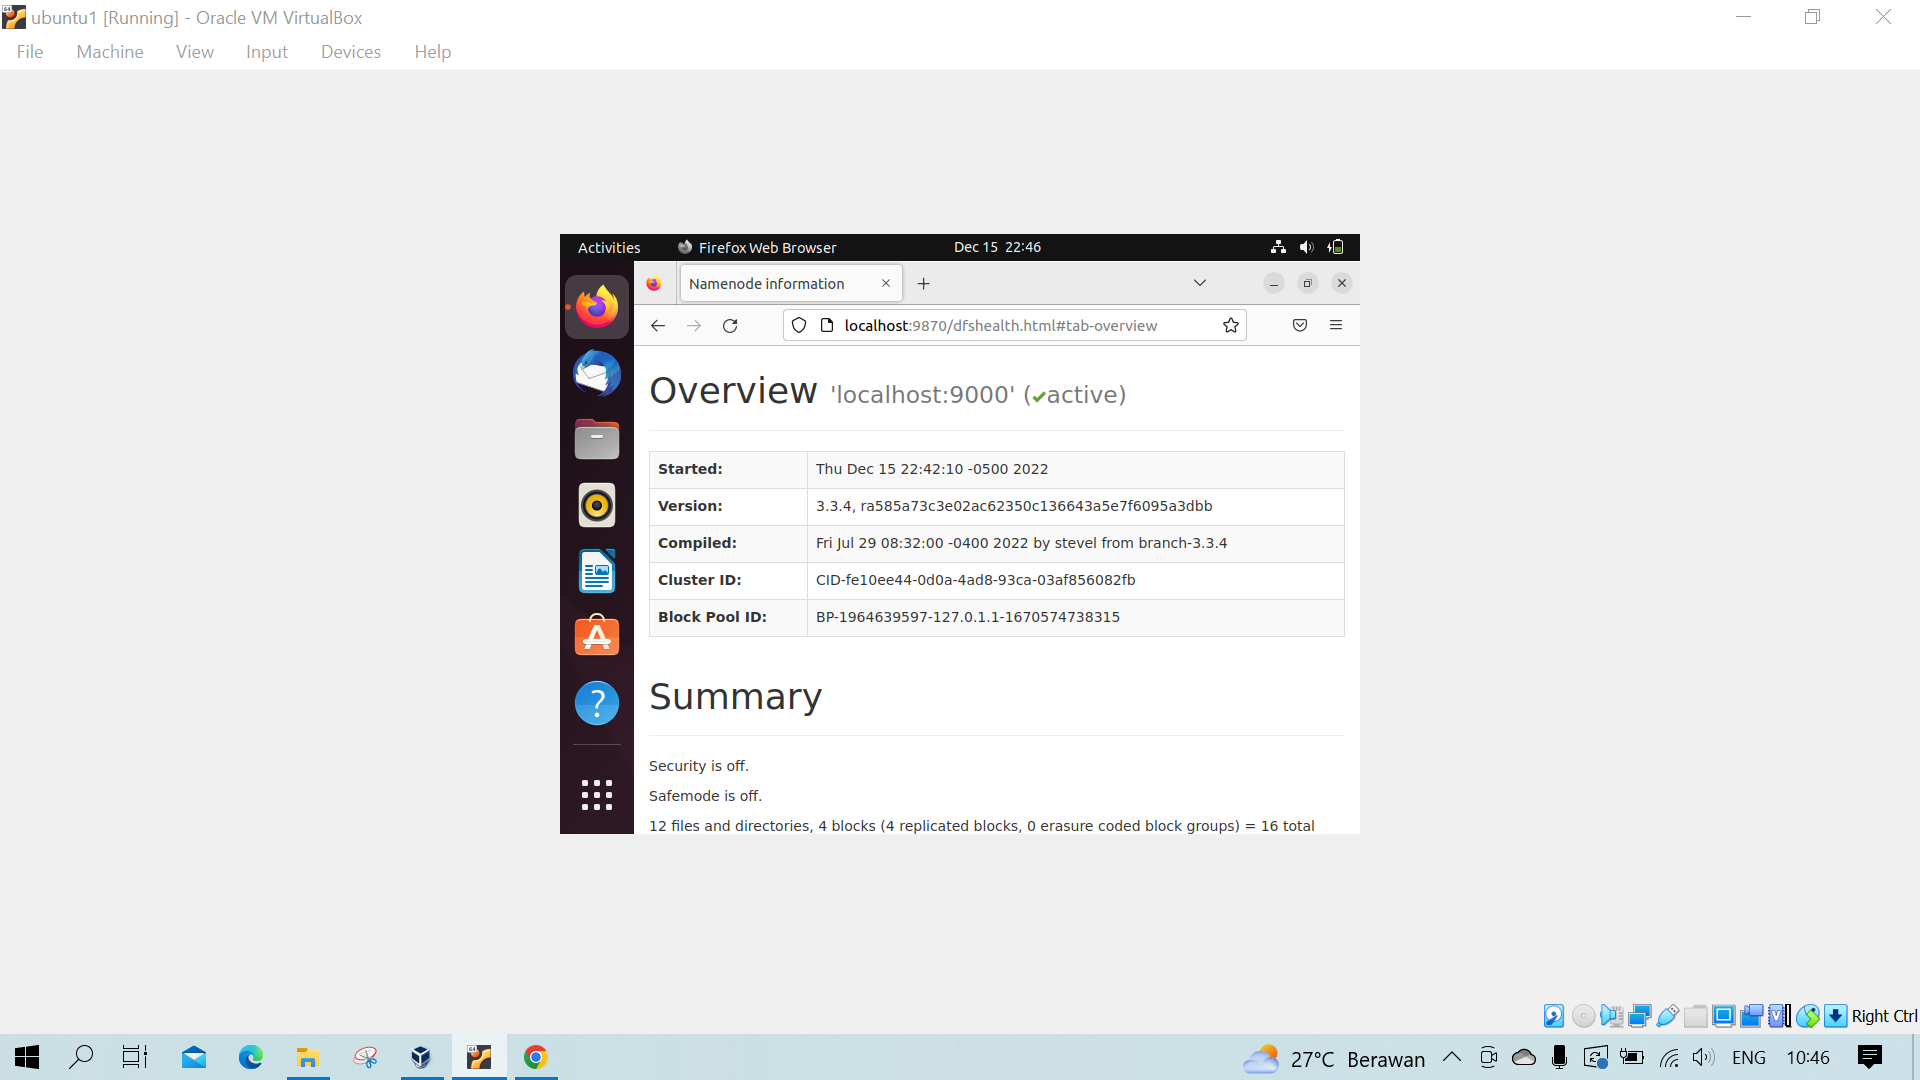
\includegraphics[width=\textwidth]{CutOpyMandalisa/01}
\caption{hasil dari cek hadoop service}
\label{gam:perkuliahan-25-11}
\end{figure}

\begin{figure}[!ht]
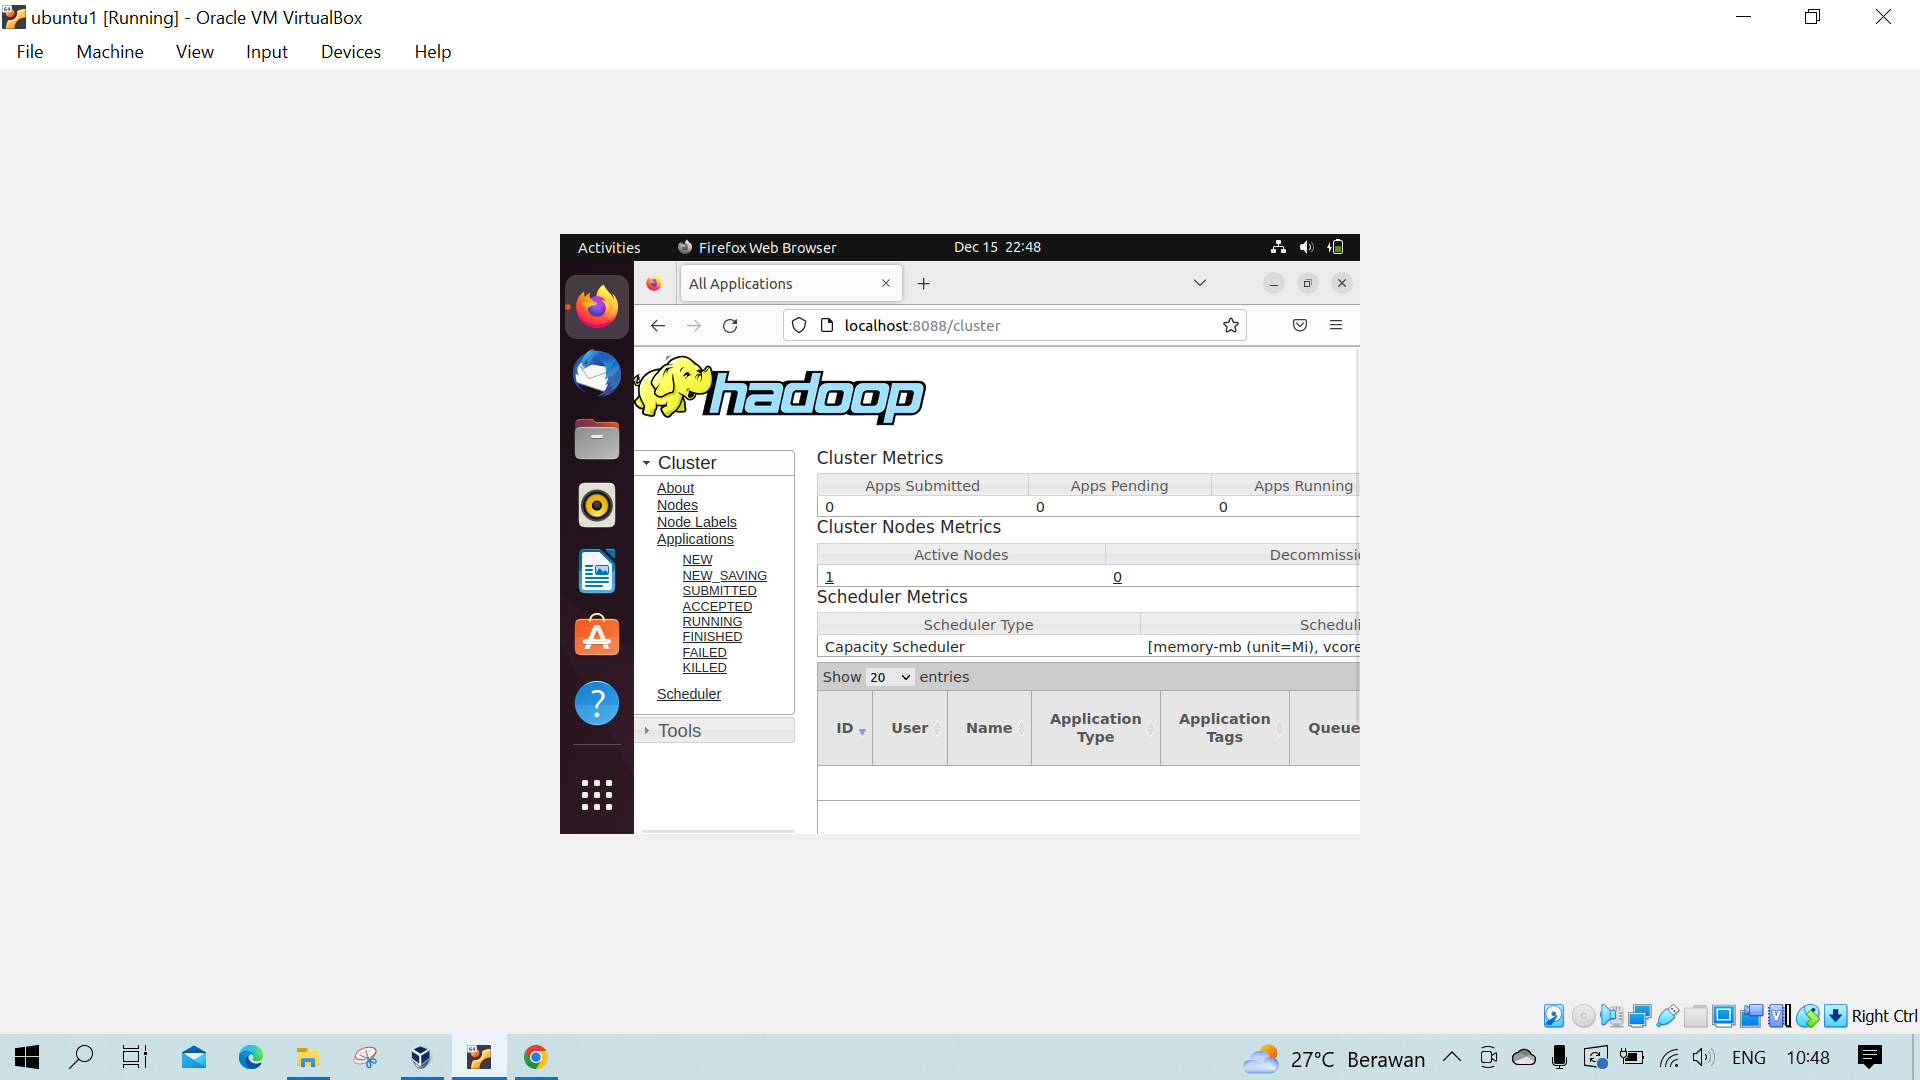
\includegraphics[width=\textwidth]{CutOpyMandalisa/02}
\caption{hasil cek hadoop service}
\label{gam:perkuliahan-25-11}
\end{figure}

\item Kesimpulan\\
% berikan kesimpulan dari praktikum yang telah dikerjkan
Behasil mendownload dan menginstal Apache hadoop dan sudah bisa dijalankan
\end{enumerate}


\newday{\textbf{08 Desember 2022-WordCount bawaan Hadoop}}
\begin{enumerate}

\item Kendala dan Solusi
\newpage
% jelaskan kendala dan penyebab yang dialami saat mengikuti praktikum serta solusi atau langkah-langkah yang telah dilakukan
Pada praktikum ini membuat program WordCount bawaan Hadoop. Pada melakukan praktikum tidak ada kendala hanya erorr dikarenakan salah memasukkan perintah.

\begin{figure}[!ht]
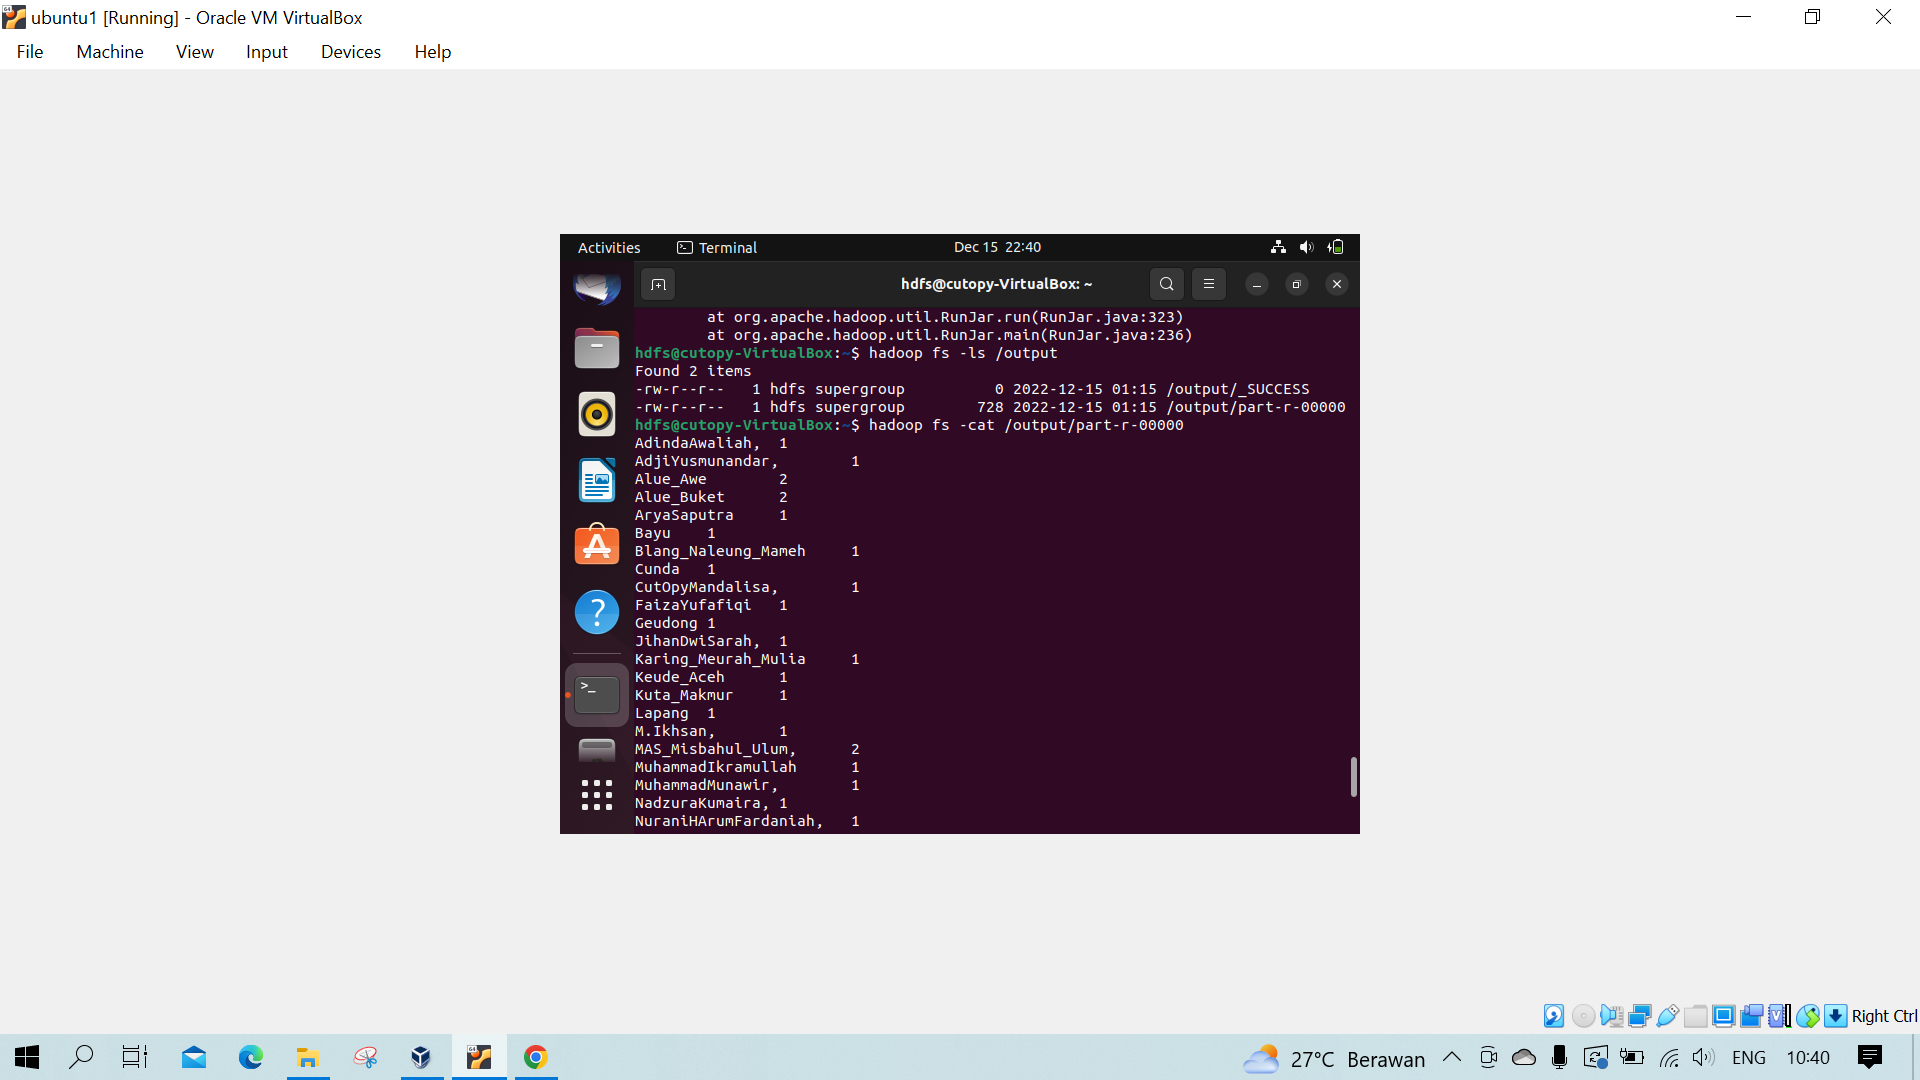
\includegraphics[width=\textwidth]{CutOpyMandalisa/03}
\caption{hasil WordCount bawaan Hadoop}
\label{gam:perkuliahan-25-11}
\end{figure}

\item Kesimpulan\\
% berikan kesimpulan dari praktikum yang telah dikerjkan
Pada praktikum ini untuk memahami proses cara kerja pada hadoop dalam memproses data input sehingga menghasilkan output.Wordcount merupakan program untuk menghitung jumlah kata dalam input.
\end{enumerate}


\newday{\textbf{09 Desember 2022-WordCount dengan Java}}
\begin{enumerate}
\item Kendala dan Solusi\\
% jelaskan kendala dan penyebab yang dialami saat mengikuti praktikum serta solusi atau langkah-langkah yang telah dilakukan
Pada praktikum ini membuat program WordCount dengan java.Pada saat melakukan praktikum terdapat error akan tetapi erorrnya disebabkan salah memasukkan perintah codingannya.solusinya harus lebih teliti saat memasukkan codingan tersebut.

\begin{figure}[!ht]
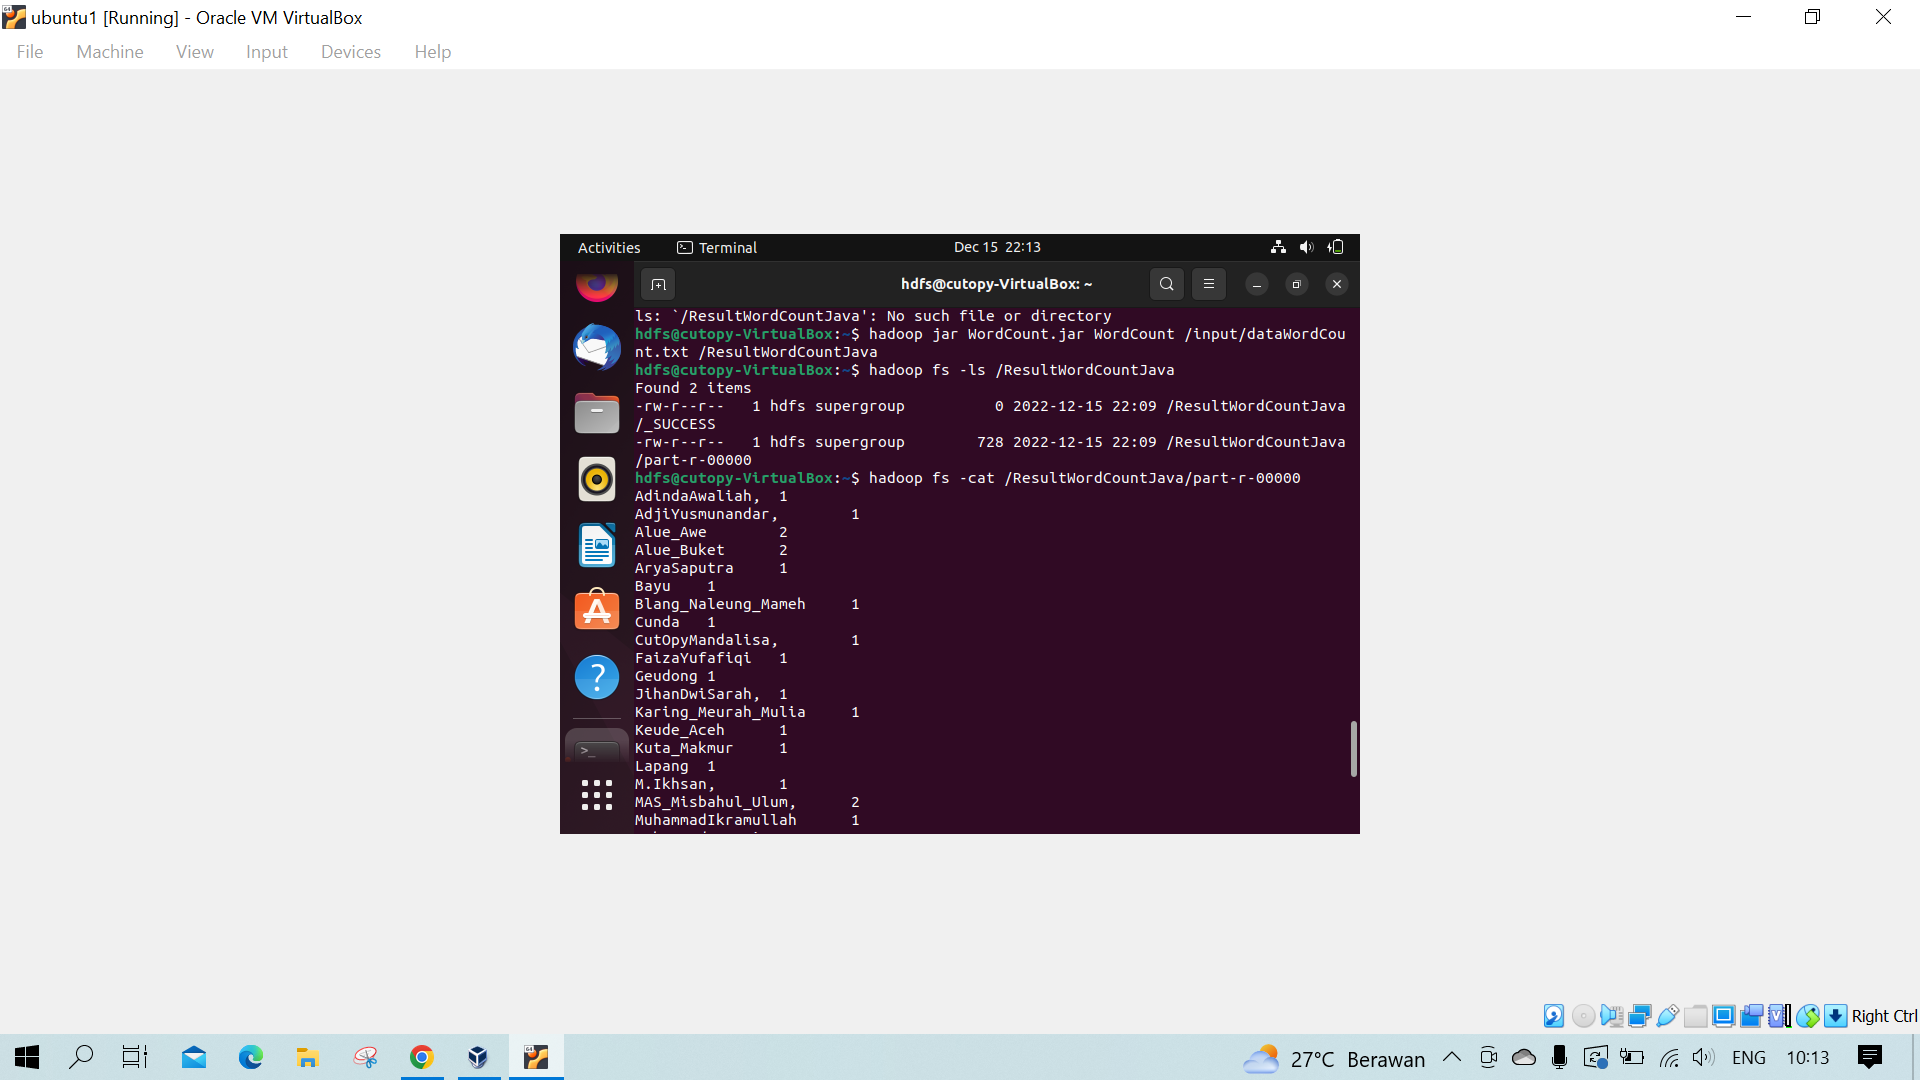
\includegraphics[width=\textwidth]{CutOpyMandalisa/04}
\caption{hasil wordCount dengan java}
\label{gam:perkuliahan-25-11}
\end{figure}

\item Kesimpulan\\
% berikan kesimpulan dari praktikum yang telah dikerjkan
Berhasil menjalankan program WordCount dengan java.
\end{enumerate}


\newday{\textbf{15 Desember 2022}}
\begin{enumerate}
\item Kendala dan Solusi
% jelaskan kendala dan penyebab yang dialami saat mengikuti praktikum serta solusi atau langkah-langkah yang telah dilakukan

\item Kesimpulan
% berikan kesimpulan dari praktikum yang telah dikerjkan
\end{enumerate}


\newday{\textbf{16 Desember 2022}}
\begin{enumerate}
\item Kendala dan Solusi
% jelaskan kendala dan penyebab yang dialami saat mengikuti praktikum serta solusi atau langkah-langkah yang telah dilakukan

\item Kesimpulan
% berikan kesimpulan dari praktikum yang telah dikerjkan
\end{enumerate}

\newday{\textbf{22 Desember 2022}}
\begin{enumerate}
\item Kendala dan Solusi
% jelaskan kendala dan penyebab yang dialami saat mengikuti praktikum serta solusi atau langkah-langkah yang telah dilakukan

\item Kesimpulan
% berikan kesimpulan dari praktikum yang telah dikerjkan
\end{enumerate}

\newday{\textbf{23 Desember 2022}}
\begin{enumerate}
\item Kendala dan Solusi
% jelaskan kendala dan penyebab yang dialami saat mengikuti praktikum serta solusi atau langkah-langkah yang telah dilakukan

\item Kesimpulan
% berikan kesimpulan dari praktikum yang telah dikerjkan
\end{enumerate}
\newthought{\textbf{Adinda Awaliah - 2020903430004 - TRKJ 3B}}

\newday{\textbf{22 September 2022}}
\begin{enumerate}
\item Kendala dan Solusi
% jelaskan kendala dan penyebab yang dialami saat mengikuti praktikum serta solusi atau langkah-langkah yang telah dilakukan

\item Kesimpulan
% berikan kesimpulan dari praktikum yang telah dikerjkan

\end{enumerate}


\newthought{\textbf{Jihan Dwi Sarah - 2020903430015 - TRKJ 3B}}


\newday{\textbf{1 - 2 Desember 2022} - Instalasi Hadoop}
\begin{enumerate}
\item Kendala dan Solusi
% jelaskan kendala dan penyebab yang dialami saat mengikuti praktikum serta solusi atau langkah-langkah yang telah dilakukan
\newline Pada pertemuan hari ini, kegiatan yang dilakukan adalah menginstall Apache Hadoop. Selama praktikum tidak mengalami kendala.

\item Kesimpulan \\
% berikan kesimpulan dari praktikum yang telah dikerjkan
Berhasil melakukan instalasi java tanpa ada bug atau error serta instalasi hadoop berikut ini gambar hasil verifikasi instalasi java version dan hadoop version 

\begin{figure}[!ht]
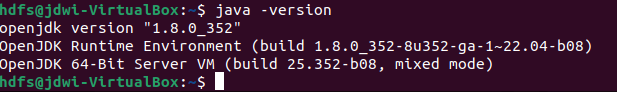
\includegraphics[width=\textwidth]{JihanDwiSarah/Java-version(Jihan)}
\caption{Verifikasi Hasil Instalasi Java}
\label{gam:Java-version(Jihan)}
\end{figure} 

\begin{figure}[!ht]
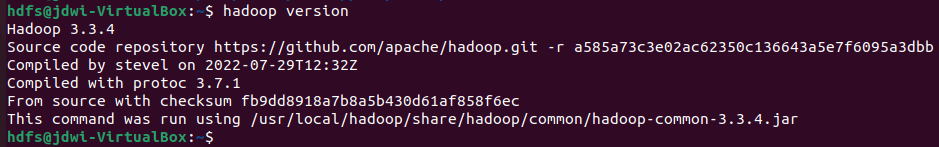
\includegraphics[width=\textwidth]{JihanDwiSarah/Hadoop-version(Jihan)}
\caption{Verifikasi Hasil Instalasi Hadoop}
\label{gam:Hadoop-version(Jihan)}
\end{figure}
\end{enumerate}


\newday{\textbf{8 - 9 Desember 2022} - Konfigurasi Hadoop}
\begin{enumerate}
\item Kendala dan Solusi \\
% jelaskan kendala dan penyebab yang dialami saat mengikuti praktikum serta solusi atau langkah-langkah yang telah dilakukan
Pada pertemuan hari ini, kegiatan yang dilakukan adalah mengkonfigurasi Apache Hadoop. Selama praktikum tidak mengalami kendala.

\item Kesimpulan \\
% berikan kesimpulan dari praktikum yang telah dikerjkan
Berhasil mengkonfigurasi beberapa file Hadoop sehingga memudahkan dalam memonitoring ekosistem Hadoop yang telah diinstall. Berikut ini gambar bukti keberhasilan praktikum. 

\begin{figure}[!ht]
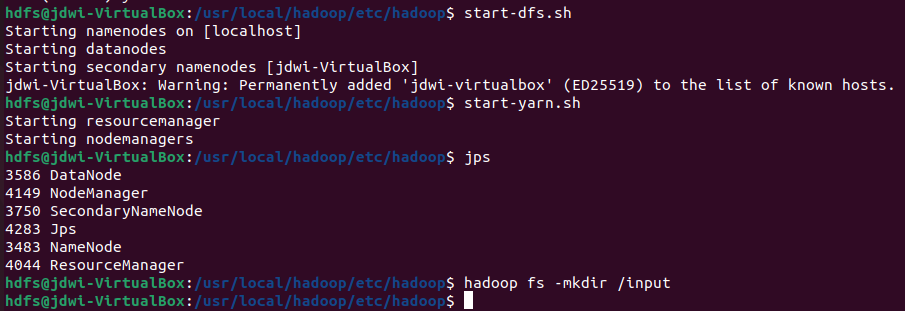
\includegraphics[width=\textwidth]{JihanDwiSarah/perintah-jps(jihan)}
\caption{Hasil perintah jps}
\label{gam:perintah-jps(jihan)}
\end{figure} 


\begin{figure}[!ht]
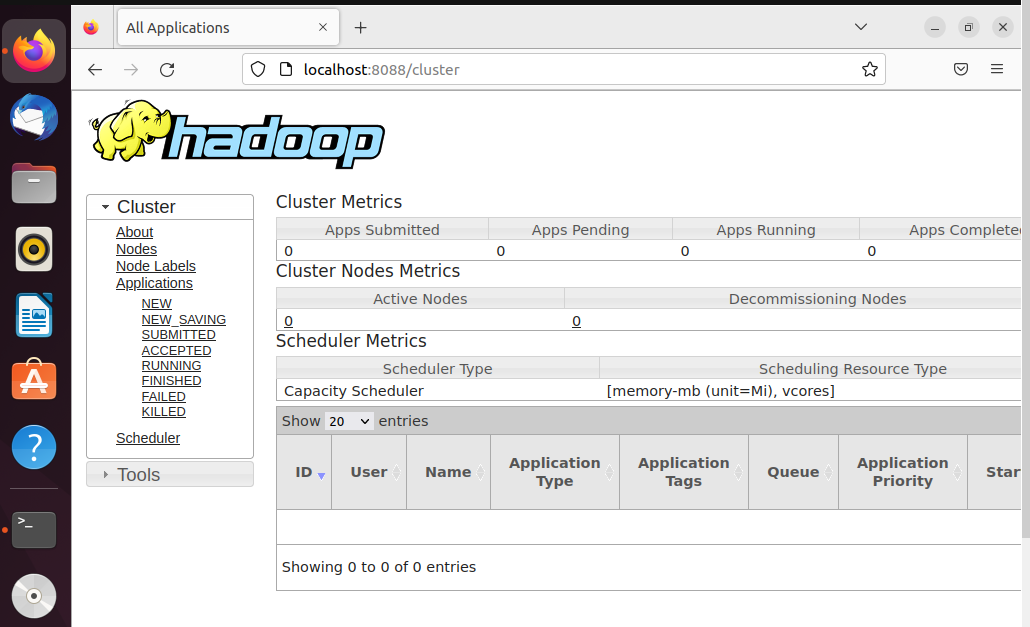
\includegraphics[width=\textwidth]{JihanDwiSarah/Akses-web-browser-8088(Jihan)}
\caption{Akses melalui web browser dengan alamat http://localhost:8088}
\label{gam:Akses-web-browser-8088(Jihan)}
\end{figure} 

\begin{figure}[!ht]
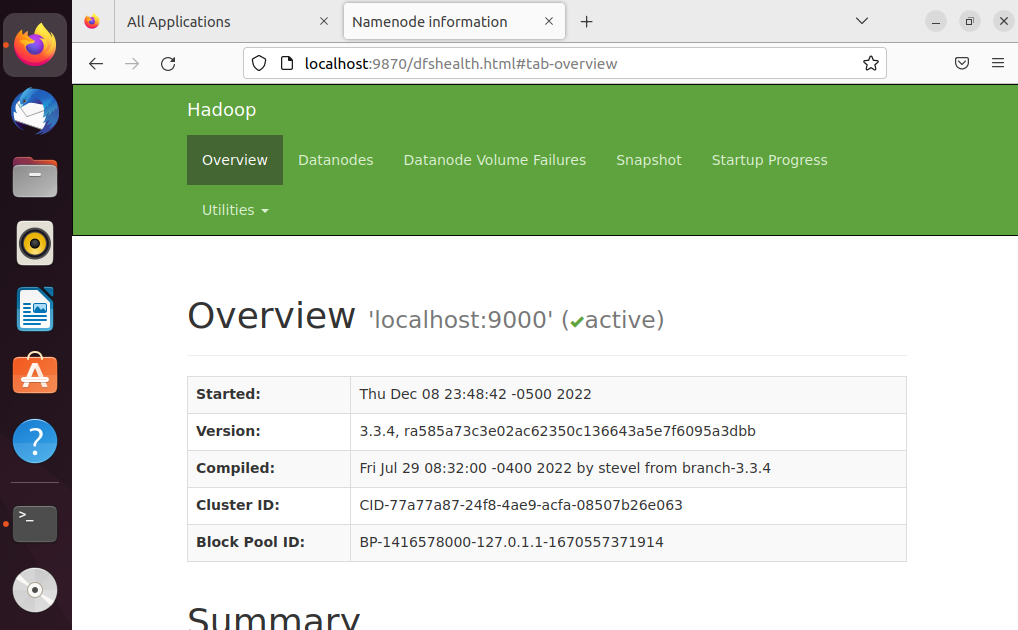
\includegraphics[width=\textwidth]{JihanDwiSarah/Akses-web-browser-9870(Jihan)}
\caption{Akses melalui web browser dengan alamat http://localhost:9870}
\label{gam:Akses-web-browser-9870(Jihan)}
\end{figure} 
\end{enumerate}

\newday{\textbf{15 Desember 2022} - WordCount Bawaan Hadoop}
\begin{enumerate}
\item Kendala dan Solusi \\
% jelaskan kendala dan penyebab yang dialami saat mengikuti praktikum serta solusi atau langkah-langkah yang telah dilakukan
Pada pertemuan hari ini, kegiatan yang dilakukan adalah mencoba program bawaan Hadoop untuk memahami bagaimana
proses dan cara kerja Hadoop dalam memproses data input hingga menghasilkan sebuah output. Selama praktikum tidak mengalami kendala.

\item Kesimpulan\\
% berikan kesimpulan dari praktikum yang telah dikerjkan
Berhasil mencoba program bawaan Hadoop yaitu program menghitung jumlah kata dalam data input yang diberikan.Berikut ini gambar bukti keberhasilan praktikum. 
\begin{figure}[!ht]
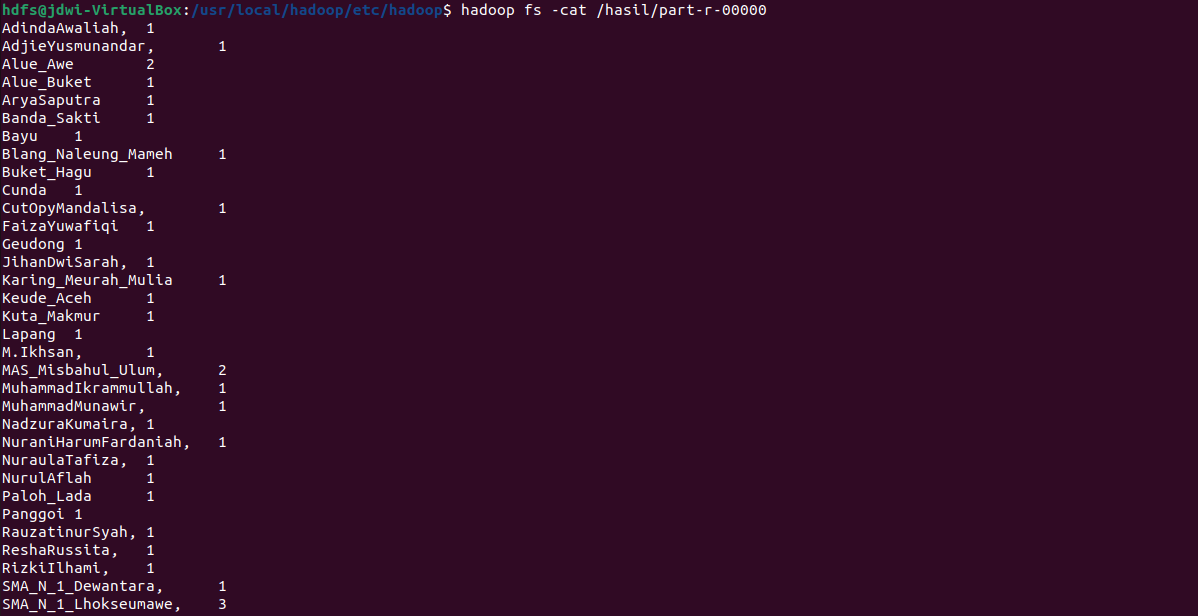
\includegraphics[width=\textwidth]{JihanDwiSarah/WordCount bawaan-Hadoop(jihan)}
\caption{Output Wordcount Bawaan Hadoop}
\label{gam:WordCount bawaan-Hadoop(jihan)}
\end{figure}
\end{enumerate}

\newday{\textbf{16 Desember 2022} - Program WordCount dengan Java}
\begin{enumerate}
\item Kendala dan Solusi \\
% jelaskan kendala dan penyebab yang dialami saat mengikuti praktikum serta solusi atau langkah-langkah yang telah dilakukan
Pada pertemuan hari ini, kegiatan yang dilakukan adalah mencoba program  wordcount dengan java. Selama praktikum mengalami kendala pada poin ke-6 berdasarkan urutan di modul. Program tidak mau dicompile karena kesalahan penulisan perintah.\\

solusinya adalah menggunakan perintah seperti berikut \\
\begin{figure}[!ht]

\includegraphics[width=\textwidth]{JihanDwiSarah/solusi-java-compile(jihan)}
\caption{Solusi Meng-Compile java}
\label{gam:solusi-java-compile(jihan)}
\end{figure}


\item Kesimpulan\\
% berikan kesimpulan dari praktikum yang telah dikerjkan
Dapat memberikan pemahaman mengenai proses membuat program wordcount java, menyiapkan data, meng-compile program hingga menjalankan program dan memperoleh hasilnya. Berikut hasil praktikum.

\begin{figure}[!ht]
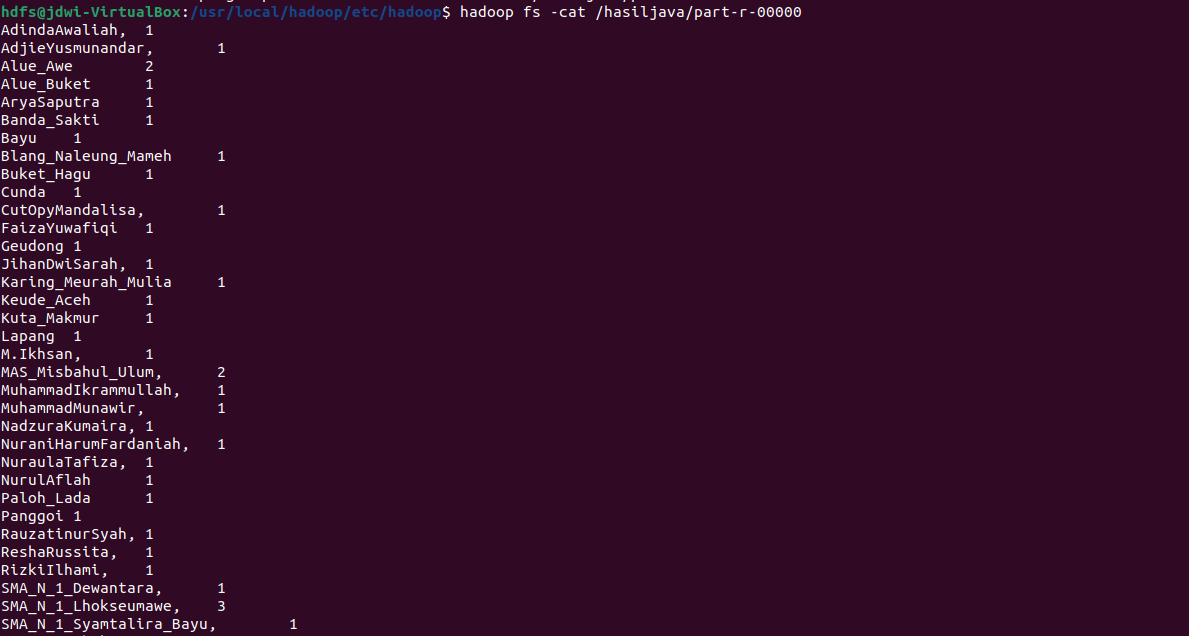
\includegraphics[width=\textwidth]{JihanDwiSarah/WordCount-Java(jihan)}
\caption{Output Wordcount java}
\label{gam:WordCount-Java(jihan)}
\end{figure}
\end{enumerate}

\newday{\textbf{17 Desember 2022} - Instalasi Apache Spark (PySpark)}
\begin{enumerate}
\item Kendala dan Solusi \\
% jelaskan kendala dan penyebab yang dialami saat mengikuti praktikum serta solusi atau langkah-langkah yang telah dilakukan
Terdapat kendala pada poin ke 3 karena kesalahan dari modulnya, perintah yang benar adalah sebagai berikut:\\
sudo mv spark-3.3.1-bin-hadoop3.\\
tidak perlu menambahkan '/usr/local/spark' lagi di akhir.


\item Kesimpulan\\
% berikan kesimpulan dari praktikum yang telah dikerjkan
Berhasil melakukan instalasi apache spark (PySpark), berikut hasil praktikum : \\

\begin{figure}[!ht]
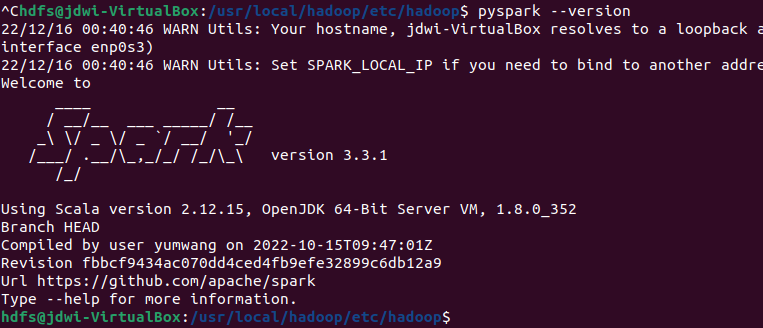
\includegraphics[width=\textwidth]{JihanDwiSarah/Instalasi-Spark(jihan)}
\caption{Hasil Instalasi Spark}
\label{gam:Instalasi-Spark(jihan)}
\end{figure}


\end{enumerate}


\newday{\textbf{22 Desember 2022} - Program WordCount dengan Python }
\begin{enumerate}
\item Kendala dan Solusi \\
% jelaskan kendala dan penyebab yang dialami saat mengikuti praktikum serta solusi atau langkah-langkah yang telah dilakukan


\item Kesimpulan\\
% berikan kesimpulan dari praktikum yang telah dikerjkan


\end{enumerate}

\newthought{\textbf{M.IKHSAN - 2020903430016 - TRKJ 3B}}

\newday{\textbf{01 Desember 2022}}
\begin{enumerate}
\item Kendala
% jelaskan kendala dan penyebab yang dialami saat mengikuti praktikum serta solusi atau langkah-langkah yang telah dilakukan
\newline 
1. saat mengintal apache hadoop, apache hadoopnya tidak selesai karena penyimpanan pada ubuntu penuh. jadi, saya menginstal ulang ubuntu untuk menambah penyimpanan
2. masih error saat menjalankan perintah start-dfs.sh 

solusi
\item Kesimpulan
% berikan kesimpulan dari praktikum yang telah dikerjkan

\end{enumerate}

\begin{figure}[!ht]
    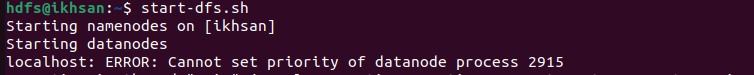
\includegraphics[width=\textwidth]{M.IKHSAN/Capture}
    \caption{error pada perintah start-hdfs.sh}
    \label{gam:Hasil}
\end{figure}

\newday{\textbf{02 Desember 2022}}
\begin{enumerate}
\item Kendala dan Solusi
% jelaskan kendala dan penyebab yang dialami saat mengikuti praktikum serta solusi atau langkah-langkah yang telah dilakukan

\item Kesimpulan
% berikan kesimpulan dari praktikum yang telah dikerjkan

\end{enumerate}

\newday{\textbf{08 Desember 2022}}
\begin{enumerate}
\item Kendala dan Solusi
% jelaskan kendala dan penyebab yang dialami saat mengikuti praktikum serta solusi atau langkah-langkah yang telah dilakukan

\item Kesimpulan
% berikan kesimpulan dari praktikum yang telah dikerjkan

\end{enumerate}


\newday{\textbf{09 Desember 2022}}
\begin{enumerate}
\item Kendala dan Solusi
% jelaskan kendala dan penyebab yang dialami saat mengikuti praktikum serta solusi atau langkah-langkah yang telah dilakukan


\item Kesimpulan
% berikan kesimpulan dari praktikum yang telah dikerjkan
\newline menginstal ulang ubuntu untuk menambah penyimpanan
\end{enumerate}

\newday{\textbf{15 Desember 2022}}
\begin{enumerate}
\item Kendala dan Solusi
% jelaskan kendala dan penyebab yang dialami saat mengikuti praktikum serta solusi atau langkah-langkah yang telah dilakukan

\item Kesimpulan
% berikan kesimpulan dari praktikum yang telah dikerjkan

\end{enumerate}

\newday{\textbf{16 Desember 2022}}
\begin{enumerate}
\item Kendala dan Solusi
% jelaskan kendala dan penyebab yang dialami saat mengikuti praktikum serta solusi atau langkah-langkah yang telah dilakukan

\item Kesimpulan
% berikan kesimpulan dari praktikum yang telah dikerjkan

\end{enumerate}

\newday{\textbf{22 Desember 2022}}
\begin{enumerate}
\item Kendala dan Solusi
% jelaskan kendala dan penyebab yang dialami saat mengikuti praktikum serta solusi atau langkah-langkah yang telah dilakukan

\item Kesimpulan
% berikan kesimpulan dari praktikum yang telah dikerjkan

\end{enumerate}

\newday{\textbf{23 Desember 2022}}
\begin{enumerate}
\item Kendala dan Solusi
% jelaskan kendala dan penyebab yang dialami saat mengikuti praktikum serta solusi atau langkah-langkah yang telah dilakukan

\item Kesimpulan
% berikan kesimpulan dari praktikum yang telah dikerjkan

\end{enumerate}
\newthought{\textbf{Adinda Awaliah - 2020903430004 - TRKJ 3B}}

\newday{\textbf{22 September 2022}}
\begin{enumerate}
\item Kendala dan Solusi
% jelaskan kendala dan penyebab yang dialami saat mengikuti praktikum serta solusi atau langkah-langkah yang telah dilakukan

\item Kesimpulan
% berikan kesimpulan dari praktikum yang telah dikerjkan

\end{enumerate}


\newthought{\textbf{Muhammad Munawir - 2020903430026 - TRKJ 3B}}

\newday{\textbf{1 September 2022}}
\begin{enumerate}
\item Kendala dan Solusi
% jelaskan kendala dan penyebab yang dialami saat mengikuti praktikum serta solusi atau langkah-langkah yang telah dilakukan

\item Kesimpulan
% berikan kesimpulan dari praktikum yang telah dikerjkan

\end{enumerate}

\newday{\textbf{2 Desember 2022}}
\begin{enumerate}
\item Kendala dan Solusi
% jelaskan kendala dan penyebab yang dialami saat mengikuti praktikum serta solusi atau langkah-langkah yang telah dilakukan

\item Kesimpulan
% berikan kesimpulan dari praktikum yang telah dikerjkan

\end{enumerate}

\newday{\textbf{8 Desember 2022}}
\begin{enumerate}
\item Kendala dan Solusi
% jelaskan kendala dan penyebab yang dialami saat mengikuti praktikum serta solusi atau langkah-langkah yang telah dilakukan

\item Kesimpulan
% berikan kesimpulan dari praktikum yang telah dikerjkan

\end{enumerate}

\newday{\textbf{9 Desember 2022}}
\begin{enumerate}
\item Kendala dan Solusi
% jelaskan kendala dan penyebab yang dialami saat mengikuti praktikum serta solusi atau langkah-langkah yang telah dilakukan

\item Kesimpulan
% berikan kesimpulan dari praktikum yang telah dikerjkan

\end{enumerate}
\newthought{\textbf{Adinda Awaliah - 2020903430004 - TRKJ 3B}}

\newday{\textbf{22 September 2022}}
\begin{enumerate}
\item Kendala dan Solusi
% jelaskan kendala dan penyebab yang dialami saat mengikuti praktikum serta solusi atau langkah-langkah yang telah dilakukan

\item Kesimpulan
% berikan kesimpulan dari praktikum yang telah dikerjkan

\end{enumerate}


\newthought{\textbf{Nurani Harum Fardaniah - 2020903430034 - TRKJ 3B}}

\newday{\textbf{1 - 2 Desember 2022} - Instalasi dan Konfigurasi Apache Hadoop}
\begin{enumerate}
\item Kendala dan Solusi \\
Kendala :\\
Saat melakukan penginstalan hadoop tidak ada kendala apapun. Namun pada saat melakukan konfigurasi hadoop terdapat kendala pada saat melakukan hdfs namenode -format. Perintah ini tidak mau dijalankan karena ada kesalahan dalam penulisan pada file core-site.xml
Saat melakukan perintah jps pun hanya menampilkan 1 saja.

Solusi :\\
Melakukan perubahan penulisan pada file core-site.xml, setelah itu perintah hdfs namenode -format dapat dijalankan dan saat melakukan perintah jps akhirnya muncul ada 5.

\item Kesimpulan \\
Praktikum penginstalan hadoop dan konfigurasi hadoop berhasil dijalankan sesuai perintah-perintah yang ada.

\begin{figure}[!ht]
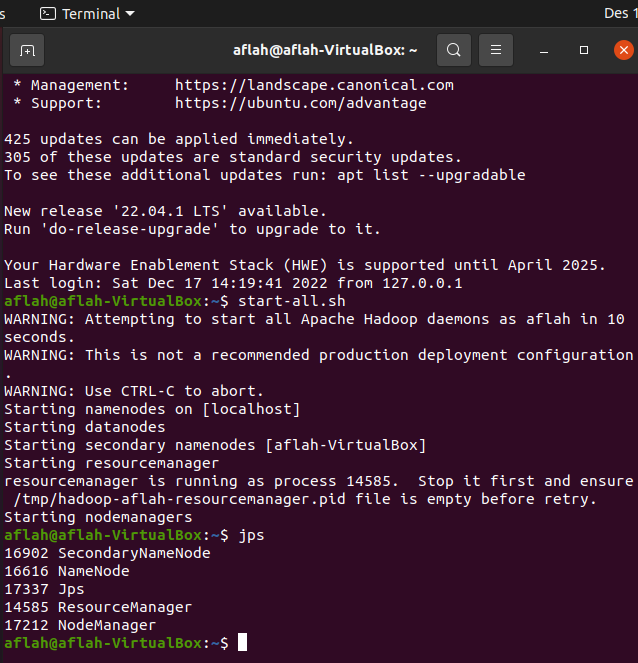
\includegraphics[width=\textwidth]{NuraniHarumFardaniah/jps}
\caption{hasil dari jps}
\label{gam:perkuliahan-25-11}
\end{figure}

\begin{figure}[!ht]
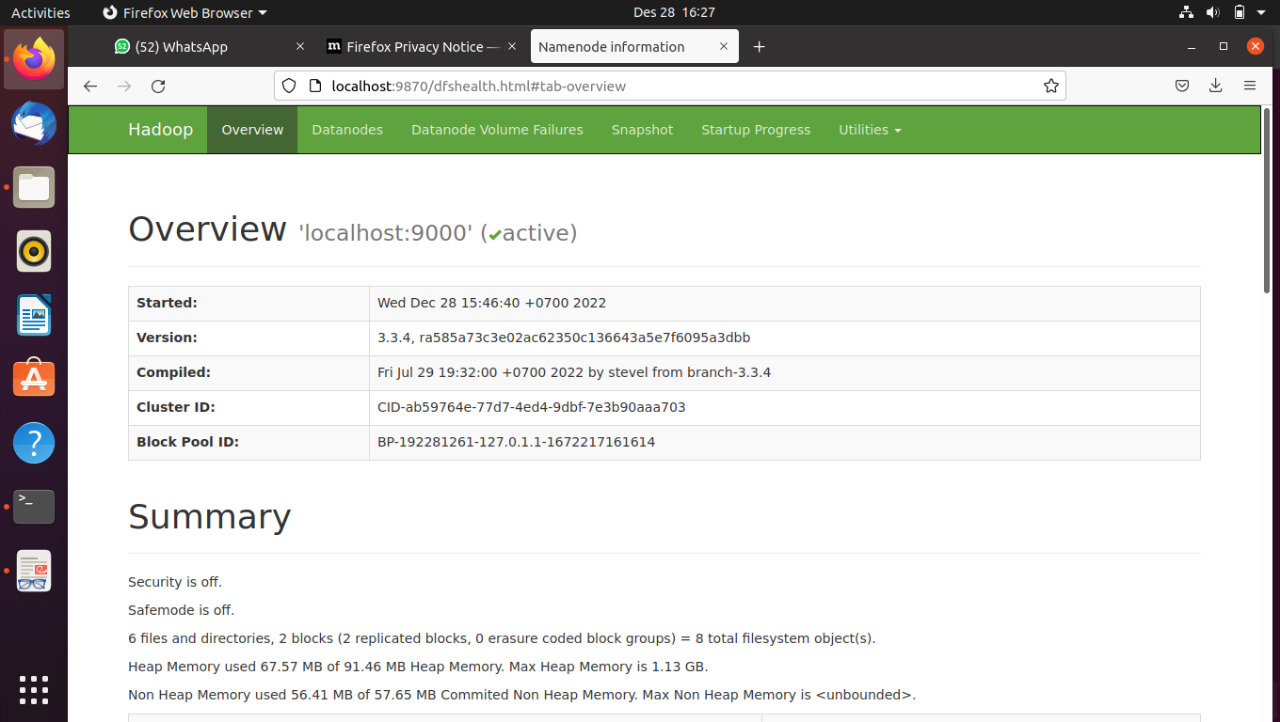
\includegraphics[width=\textwidth]{NuraniHarumFardaniah/localhost9870}
\caption{hasil dari localhost 9870}
\label{gam:perkuliahan-25-11}
\end{figure}

\newpage
\begin{figure}[!ht]
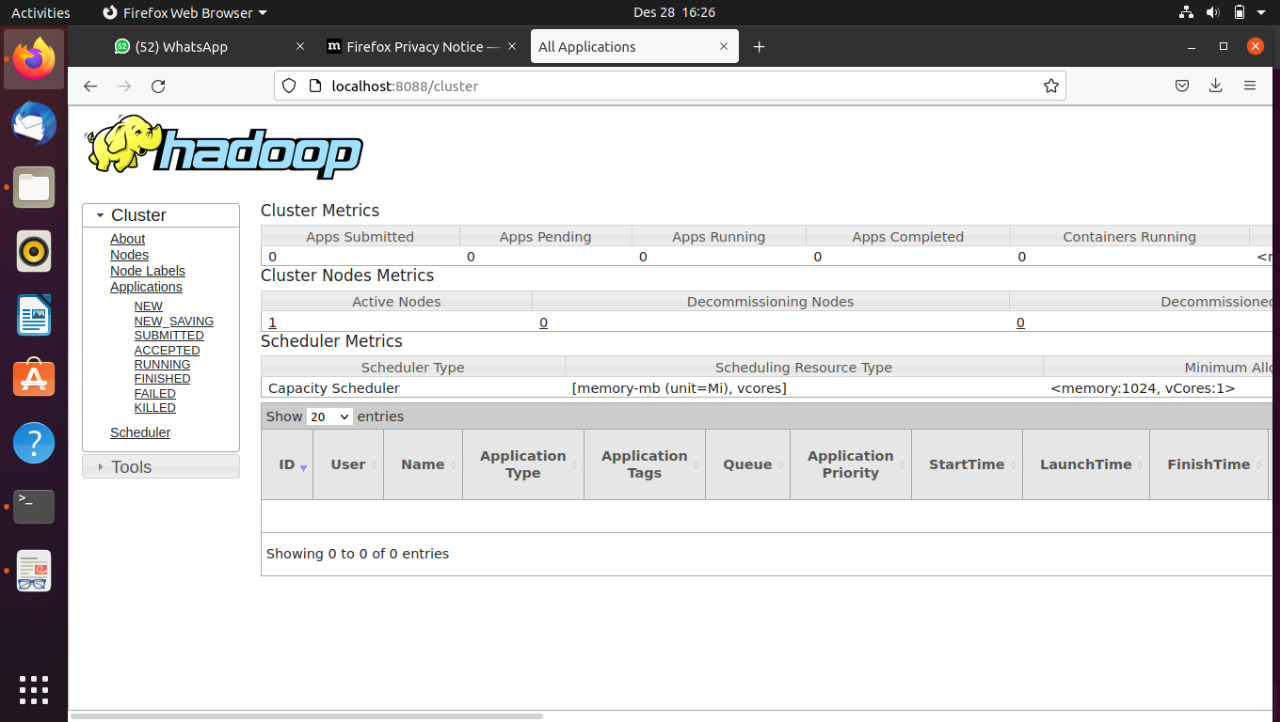
\includegraphics[width=\textwidth]{NuraniHarumFardaniah/localhost8088}
\caption{hasil dari localhost 8088}
\label{gam:perkuliahan-25-11}
\end{figure}

\end{enumerate}

\newday{\textbf{8 Desember 2022} - WordCount Bawaan Java}
\begin{enumerate}
\item Kendala dan Solusi
\newline Tidak ada kendala apapun saat melakukan program WordCount bawaan Hadoop

\item Kesimpulan
\newline Praktikum berhasil dilakukan sesuai dengan perintah-perintah yang ada. WordCount sendiri merupakan program untuk menghitung jumlah kata yang ada pada data.


\begin{figure}[!ht]
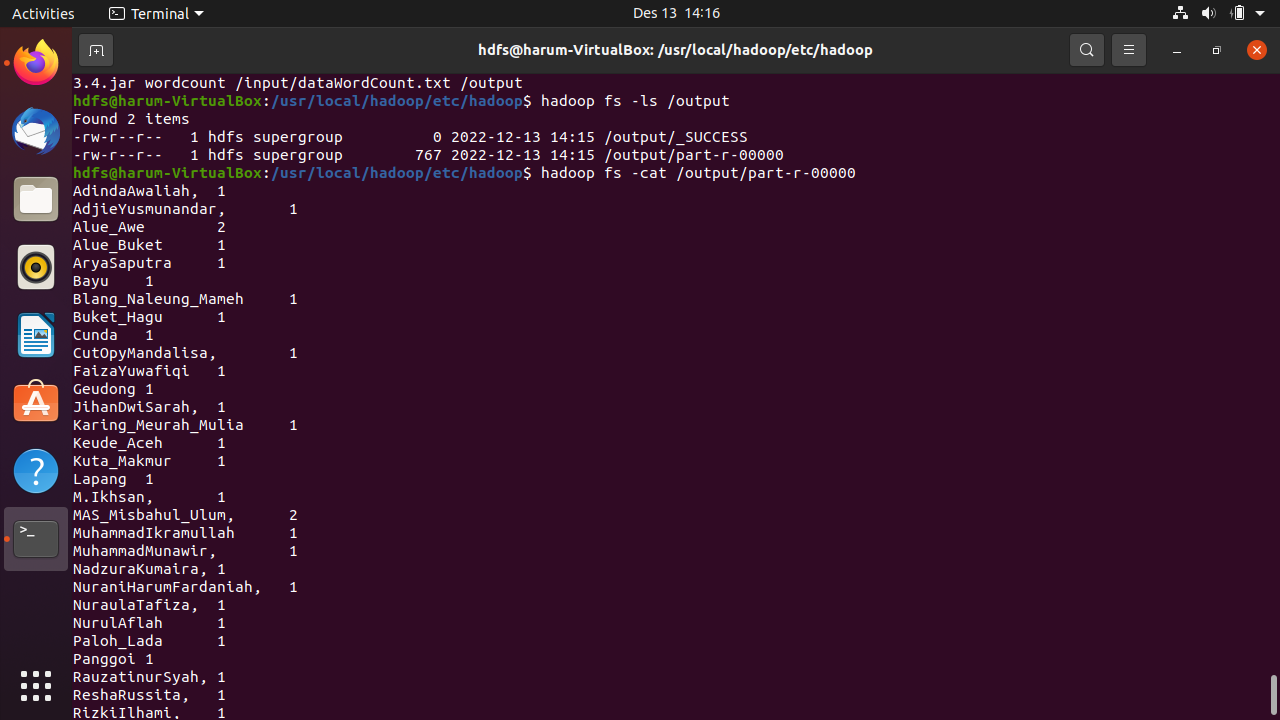
\includegraphics[width=\textwidth]{NuraniHarumFardaniah/6-7a}
\caption{Hasil dari langkah 6 dan 7}
\label{gam:perkuliahan-25-11}
\end{figure}
\newpage
\begin{figure}[!ht]
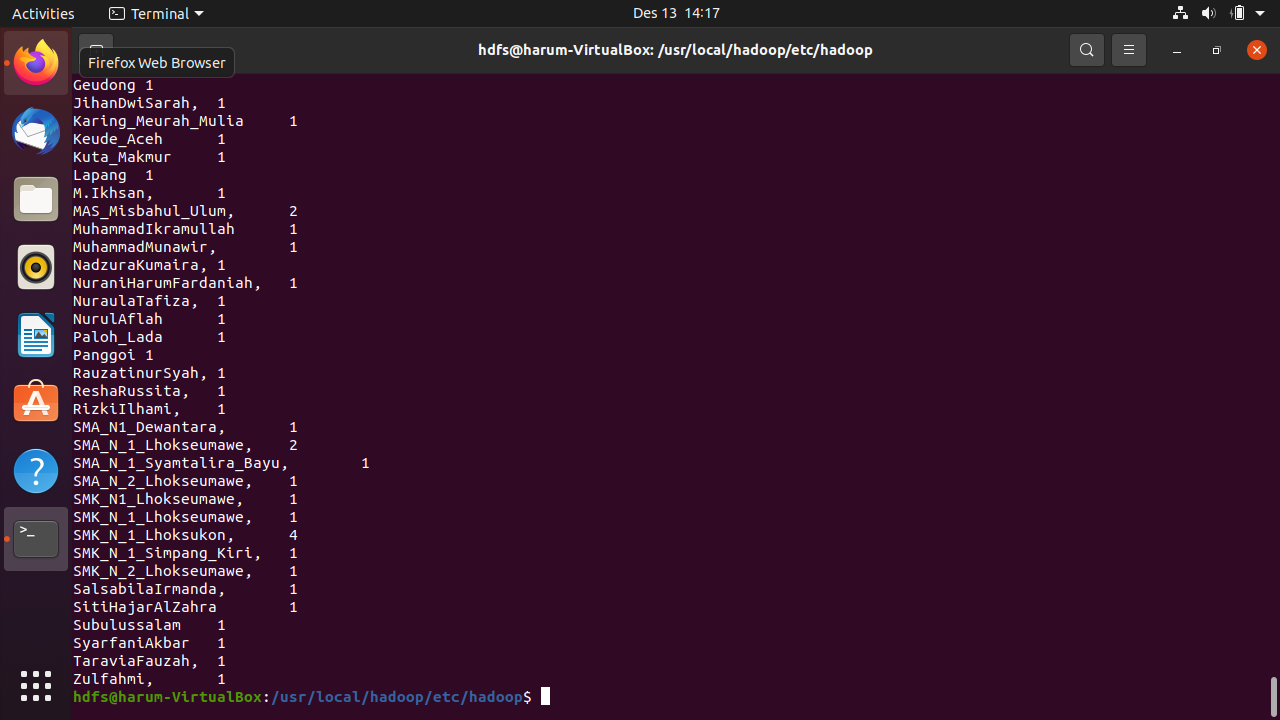
\includegraphics[width=\textwidth]{NuraniHarumFardaniah/7b}
\caption{Hasil dari langkah 7}
\label{gam:perkuliahan-25-11}
\end{figure}

\end{enumerate}

\newday{\textbf{9 Desember 2022} - WordCount dengan Java}
\begin{enumerate}
\item Kendala dan Solusi
\newline Kendala :\\
Saat melakukan praktikum program WordCount dengan Java terdapat kendala pada saat melakukan compile file WordCount. Perintah ini tidak mau dijalankan karena ada kesalahan dalam penulisan pada file WordCount.java

Solusi :\\
Melakukan perubahan penulisan pada file WordCount.java, setelah itu perintah untuk melakukan compile pada file WordCount.java dapat dijalankan.

\item Kesimpulan
\newline Praktikum berhasil dilakukan sesuai dengan perintah-perintah yang ada. Data pada WordCount dapat ditampilkan sesuai dengan yang telah dibuat.


\begin{figure}[!ht]
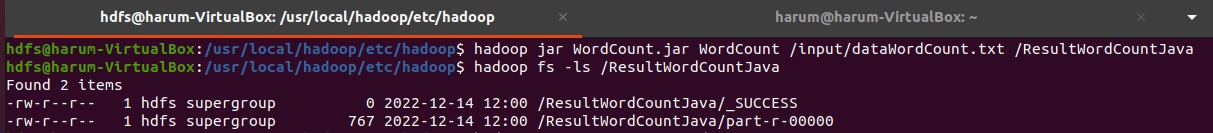
\includegraphics[width=\textwidth]{NuraniHarumFardaniah/9}
\caption{Hasil Perhitungan dengan WordCount Hadoop}
\label{gam:perkuliahan-25-11}
\end{figure}

\begin{figure}[!ht]
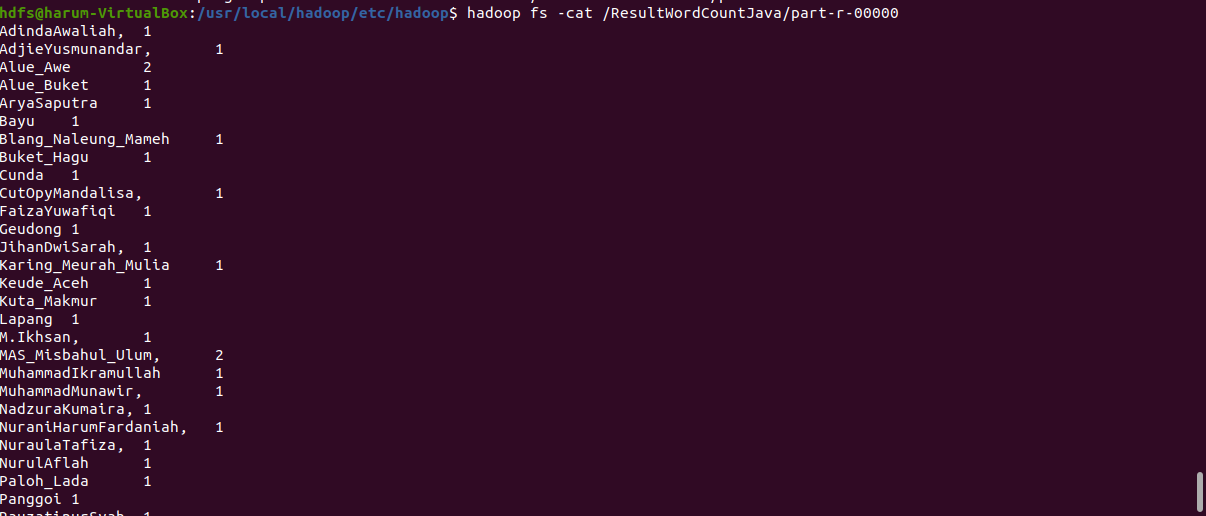
\includegraphics[width=\textwidth]{NuraniHarumFardaniah/10a}
\caption{Hasil Perhitungan dengan WordCount Hadoop}
\label{gam:perkuliahan-25-11}
\end{figure}
\newpage
\begin{figure}[!ht]
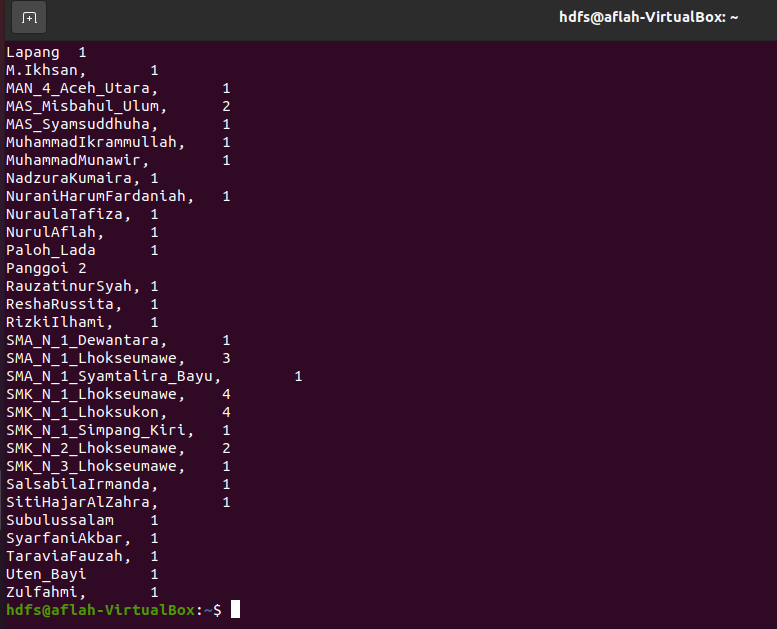
\includegraphics[width=\textwidth]{NuraniHarumFardaniah/10b}
\caption{Hasil Perhitungan dengan WordCount Hadoop}
\label{gam:perkuliahan-25-11}
\end{figure}

\end{enumerate}

\newday{\textbf{15 Desember 2022}} 
\begin{enumerate}
\item Kendala dan Solusi

\item Kesimpulan

\end{enumerate}
\newthought{\textbf{Adinda Awaliah - 2020903430004 - TRKJ 3B}}

\newday{\textbf{22 September 2022}}
\begin{enumerate}
\item Kendala dan Solusi
% jelaskan kendala dan penyebab yang dialami saat mengikuti praktikum serta solusi atau langkah-langkah yang telah dilakukan

\item Kesimpulan
% berikan kesimpulan dari praktikum yang telah dikerjkan

\end{enumerate}


\newthought{\textbf{Adinda Awaliah - 2020903430004 - TRKJ 3B}}

\newday{\textbf{22 September 2022}}
\begin{enumerate}
\item Kendala dan Solusi
% jelaskan kendala dan penyebab yang dialami saat mengikuti praktikum serta solusi atau langkah-langkah yang telah dilakukan

\item Kesimpulan
% berikan kesimpulan dari praktikum yang telah dikerjkan

\end{enumerate}


\newthought{\textbf{Rauzatinur Syah - 2020903430039 - TRKJ 3B}}


\newday{\textbf{1 - 2 Desember 2022} - Instalasi dan Konfigurasi Hadoop}
\begin{enumerate}
\item Kendala dan Solusi\\
% jelaskan kendala dan penyebab yang dialami saat mengikuti praktikum serta solusi atau langkah-langkah yang telah dilakukan
\begin{enumerate}
\item Kendala
\begin{itemize}
\item terdapat kendala pada instalasi hadoop pada pengecekanan versi hadoop yang berfungsi untuk menverifikasi instalasi hadoop
\item terdapat kendala saat menjalanakn format HDFS dan hadoop service
\end{itemize}
\item Solusi \\
\begin{itemize}
\item melakukan pengecekan pada file hadoop-env.sh
\item melakuka  pengecekan pada file core-site.xml, hdfs-site.xml, mapred-site.xml, yarn-site.xml
\end{itemize}
\end{enumerate}

\item Kesimpulan\\
% berikan kesimpulan dari praktikum yang telah dikerjkan
adapun kesimpulan yang diperoleh yaitu instalasi dan konfigurasi hadoop berhasil 
\end{enumerate}

\begin{figure}[!ht]
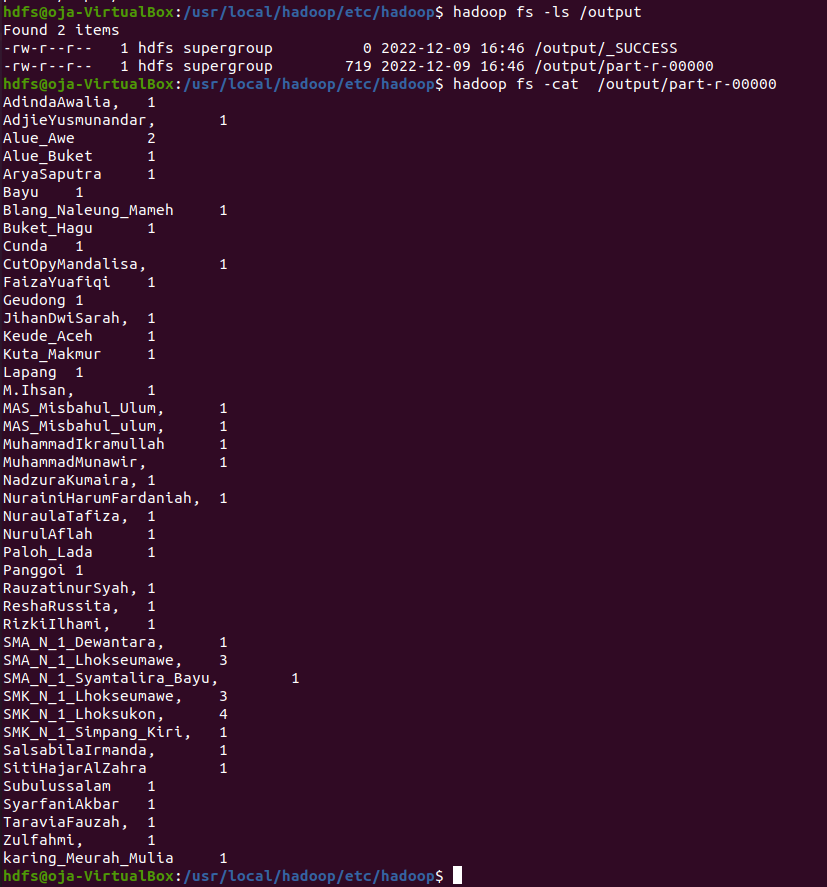
\includegraphics[width=\textwidth]{RauzatinurSyah/dataHadoop}
\caption{hasil program WordCount hadoop}
\label{gam:Hasil}
\end{figure}

\newday{\textbf{8 Desember 2022} - WordCount bawaan Hadoop}
\begin{enumerate}
\item Kendala dan Solusi\\
% jelaskan kendala dan penyebab yang dialami saat mengikuti praktikum serta solusi atau langkah-langkah yang telah dilakukan
pada pratikum Program WordCount bawaan hadoop tidak ada kendala pada praktikum yang dilakukan
\item Kesimpulan\\
% berikan kesimpulan dari praktikum yang telah dikerjkan
berhasil menjalanakan program wordCount bawan hadoop
\end{enumerate}


\begin{figure}[!ht]
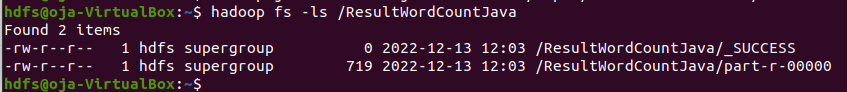
\includegraphics[width=\textwidth]{RauzatinurSyah/datahadoopjava no 9}
\caption{hasil program WordCount java no.9}
\label{gam:hasil program}
\end{figure}

\begin{figure}[!ht]
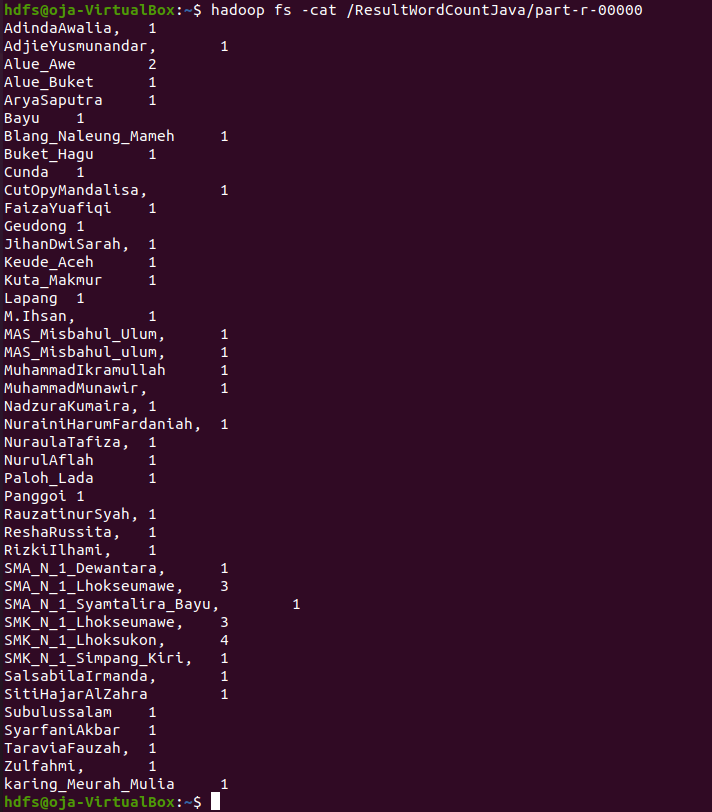
\includegraphics[width=\textwidth]{RauzatinurSyah/datahadoopjava no 10}
\caption{hasil program WordCount java no.10}
\label{gam:hasil program}
\end{figure}

\newday{\textbf{9 Desember 2022} - WordCount dengan Java}
\begin{enumerate}
\item Kendala dan Solusi \\
% jelaskan kendala dan penyebab yang dialami saat mengikuti praktikum serta solusi atau langkah-langkah yang telah dilakukan
pada praktikum WordCount dengan java
\begin{enumerate}
\item kendala: \\
terdapat kendala pada perintah menjalankan program dengan perintah"hadoop jar WordCount.jar WordCount /input/data/WordCount.txt /ResultWourdCountJava"
\item solusi: \\
menjalankan hadoop service dengan perintah "start-all.sh" dikarnakan terdapat kesalahan yang dilakukan yaitu tidak menjalankan hadoop service
\end{enumerate}
\item Kesimpulan\\
% berikan kesimpulan dari praktikum yang telah dikerjkan
adapun kesimpulan yang diperoleh yaitu berhasil menjalankan programa tersebut 
\end{enumerate}

\newday{\textbf{15 Desember 2022}}
\begin{enumerate}
\item Kendala dan Solusi\\
% jelaskan kendala dan penyebab yang dialami saat mengikuti praktikum serta solusi atau langkah-langkah yang telah dilakukan
pada instalasi apache spark tidak ada kendala yang dialami 
\item Kesimpulan\\
% berikan kesimpulan dari praktikum yang telah dikerjkan
apache spark berhasil dijalankan

\end{enumerate}

\begin{figure}[!ht]
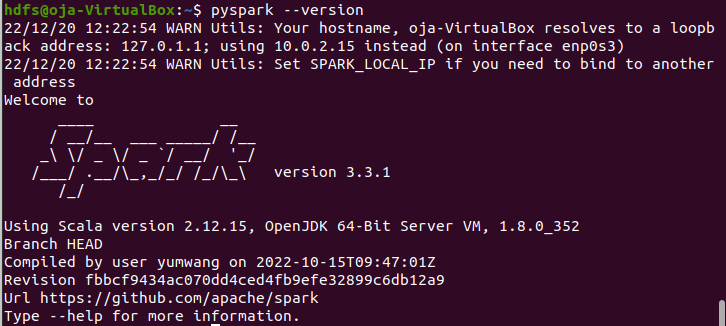
\includegraphics[width=\textwidth]{RauzatinurSyah/install spark}
\caption{hasil instalasi apache spark }
\label{gam:hasil instalasi spark}
\end{figure}


\newday{\textbf{16 Desember 2022}}
\begin{enumerate}
\item Kendala dan Solusi
% jelaskan kendala dan penyebab yang dialami saat mengikuti praktikum serta solusi atau langkah-langkah yang telah dilakukan

\item Kesimpulan
% berikan kesimpulan dari praktikum yang telah dikerjkan

\end{enumerate}

\newthought{\textbf{Resha Russita - 2020903430040 - TRKJ 3B}}

\newday{\textbf{22 September 2022}}
\begin{enumerate}
\item Kendala dan Solusi
Pada Instalasi Apache Hadoop, saya sebagai praktikan mengalami kendala saat mengekstrak file Apache Hadoop. Solusi yang saya gunakan adalah membuat kembali os ubuntu dengan ukuran ruang yang lebih besar dari sebelumnya sehingga file yang diekstrak berhasil. 
Kendala lain yang terjadi adalah hanya kurang teliti saat melakukan konfigurasi pada Apache Hadoop.

\begin{figure}[!ht]
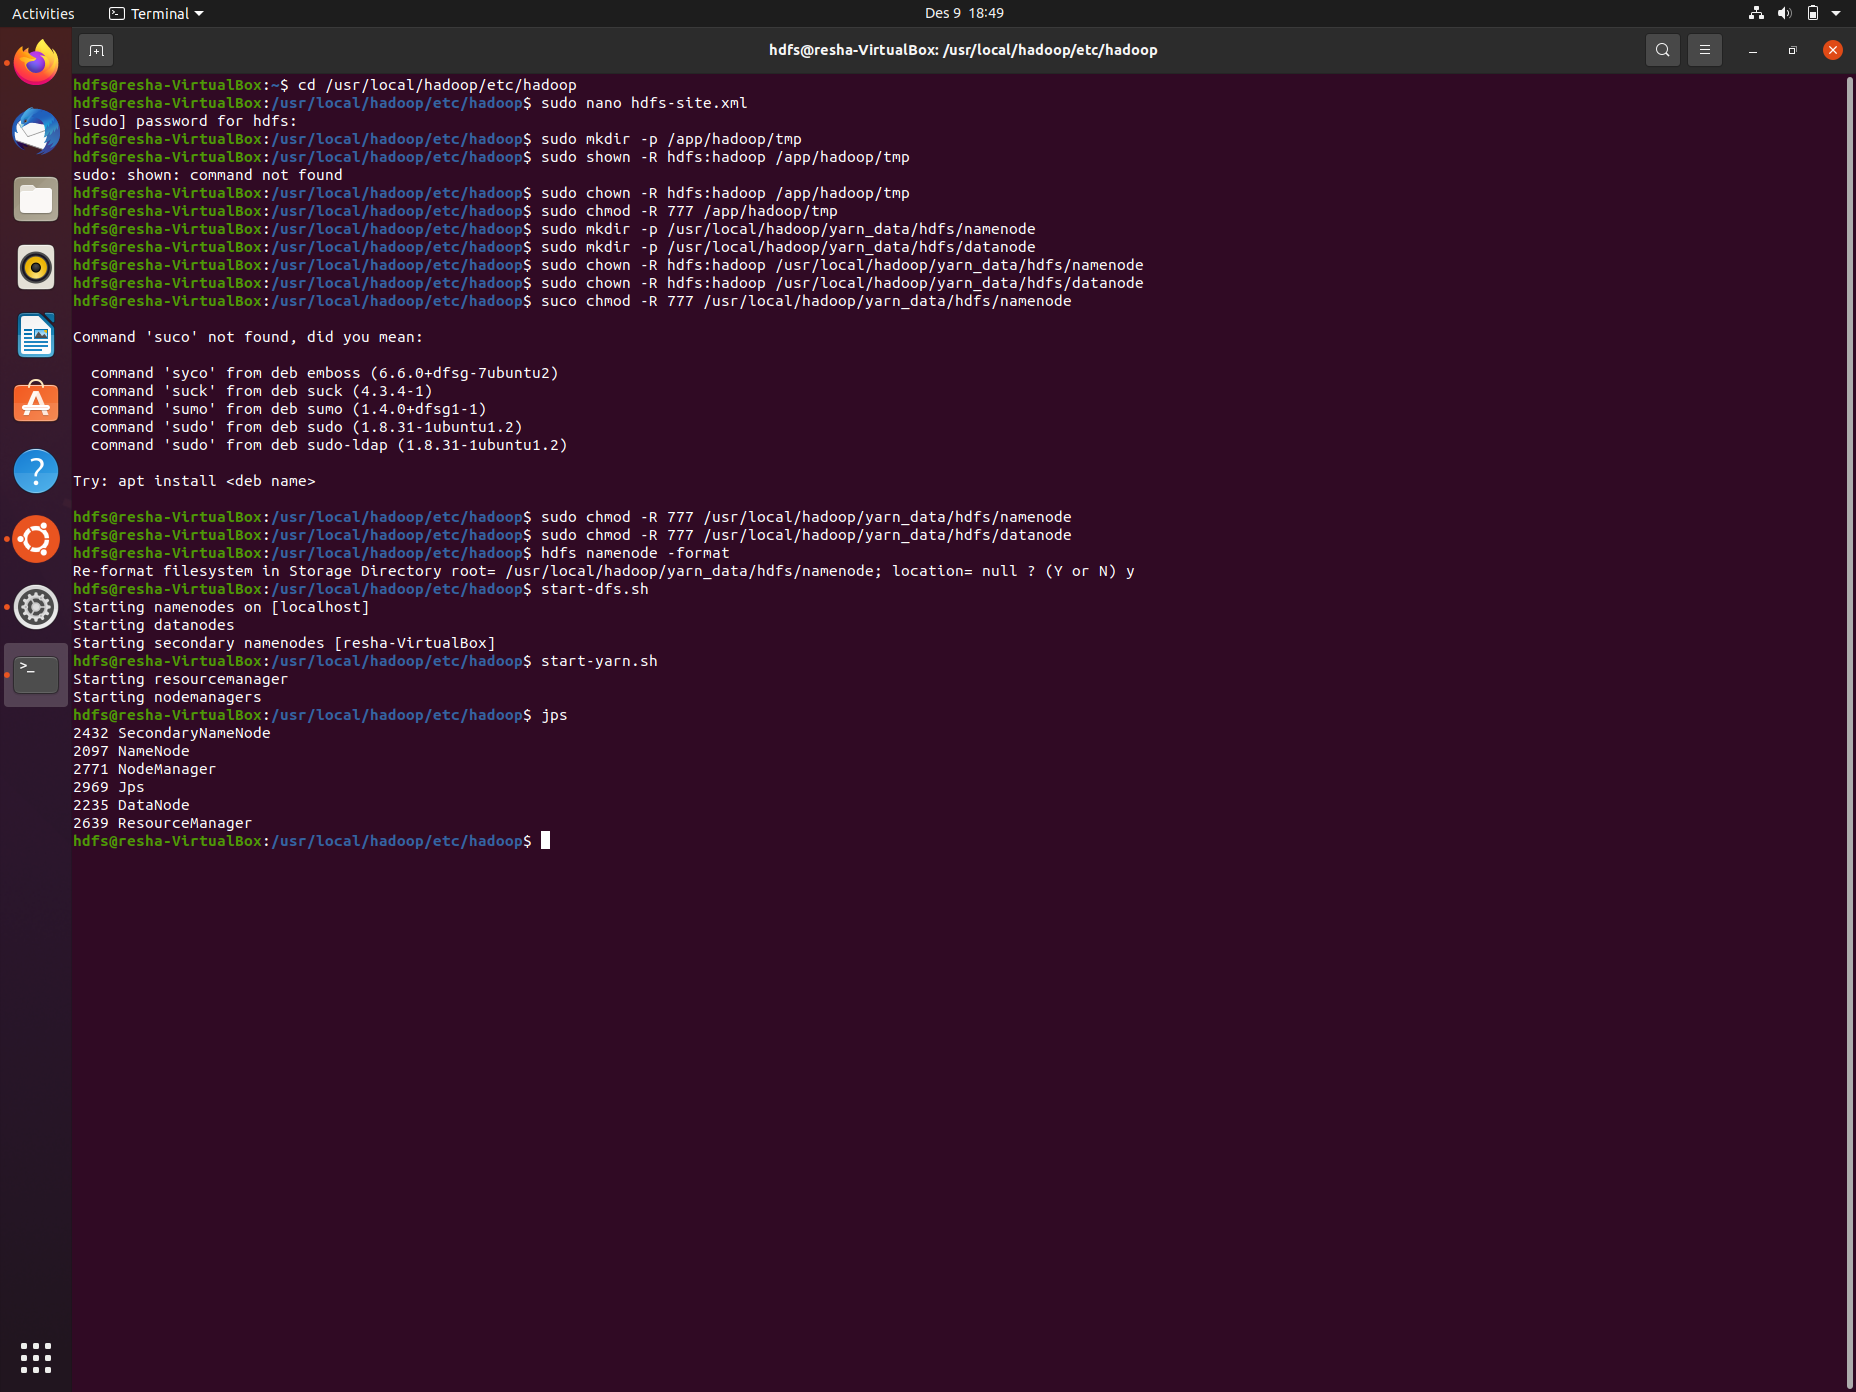
\includegraphics[width=\textwidth]{jpshadoopservice-resha}
\caption{cek services hadoop dengan jps}
\label{gam:perkuliahan-22-09}
\end{figure}

\begin{figure}[!ht]
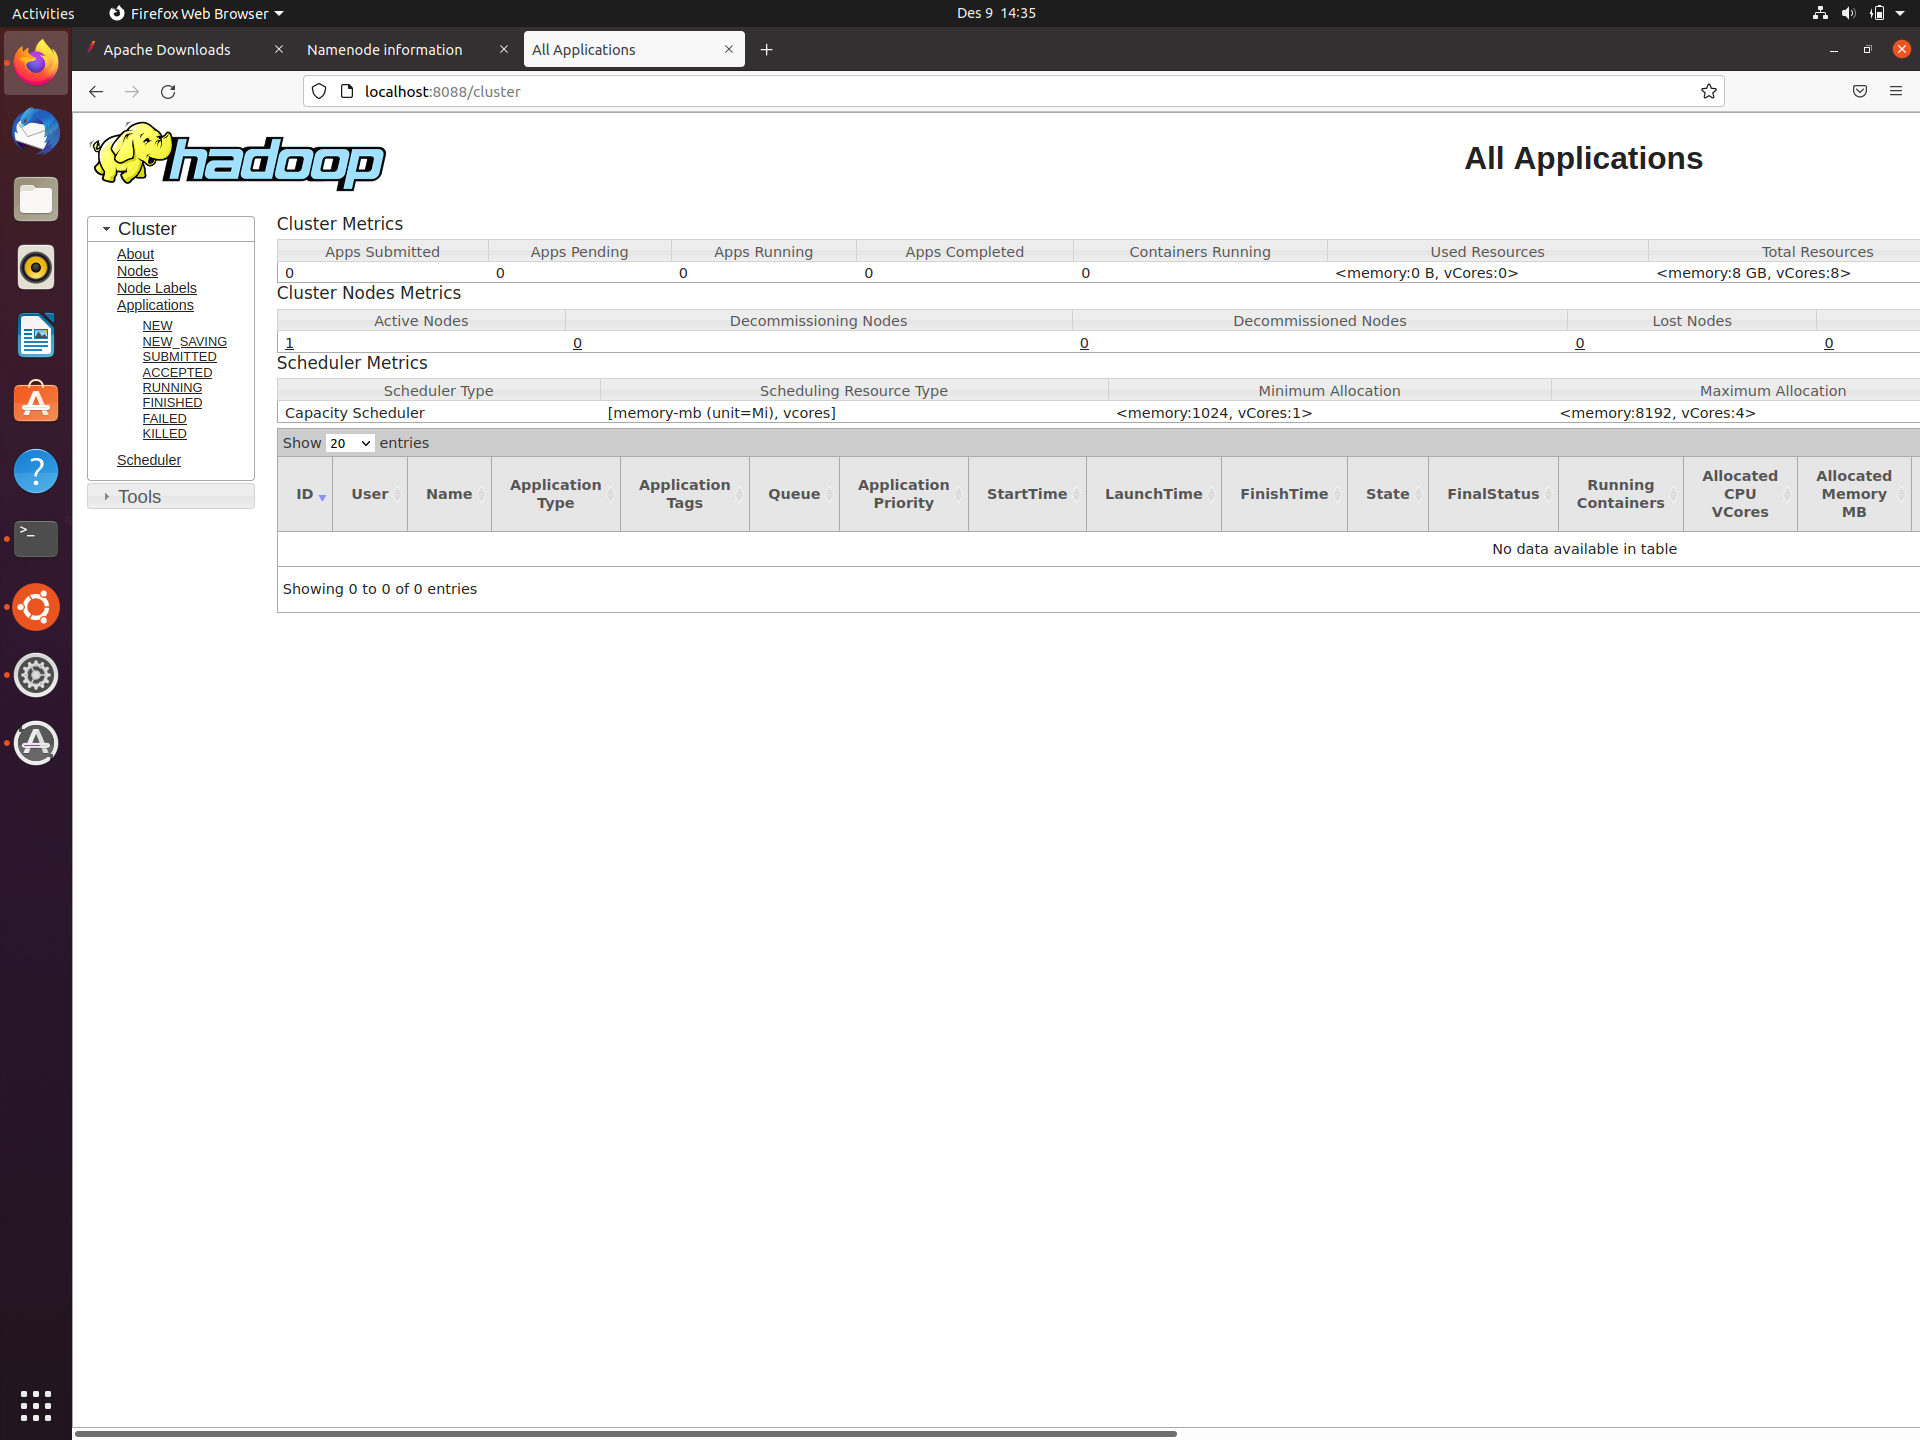
\includegraphics[width=\textwidth]{localhost8088-resha}
\caption{local host 8088 akses}
\label{gam:perkuliahan-22-09}
\end{figure}

\begin{figure}[!ht]
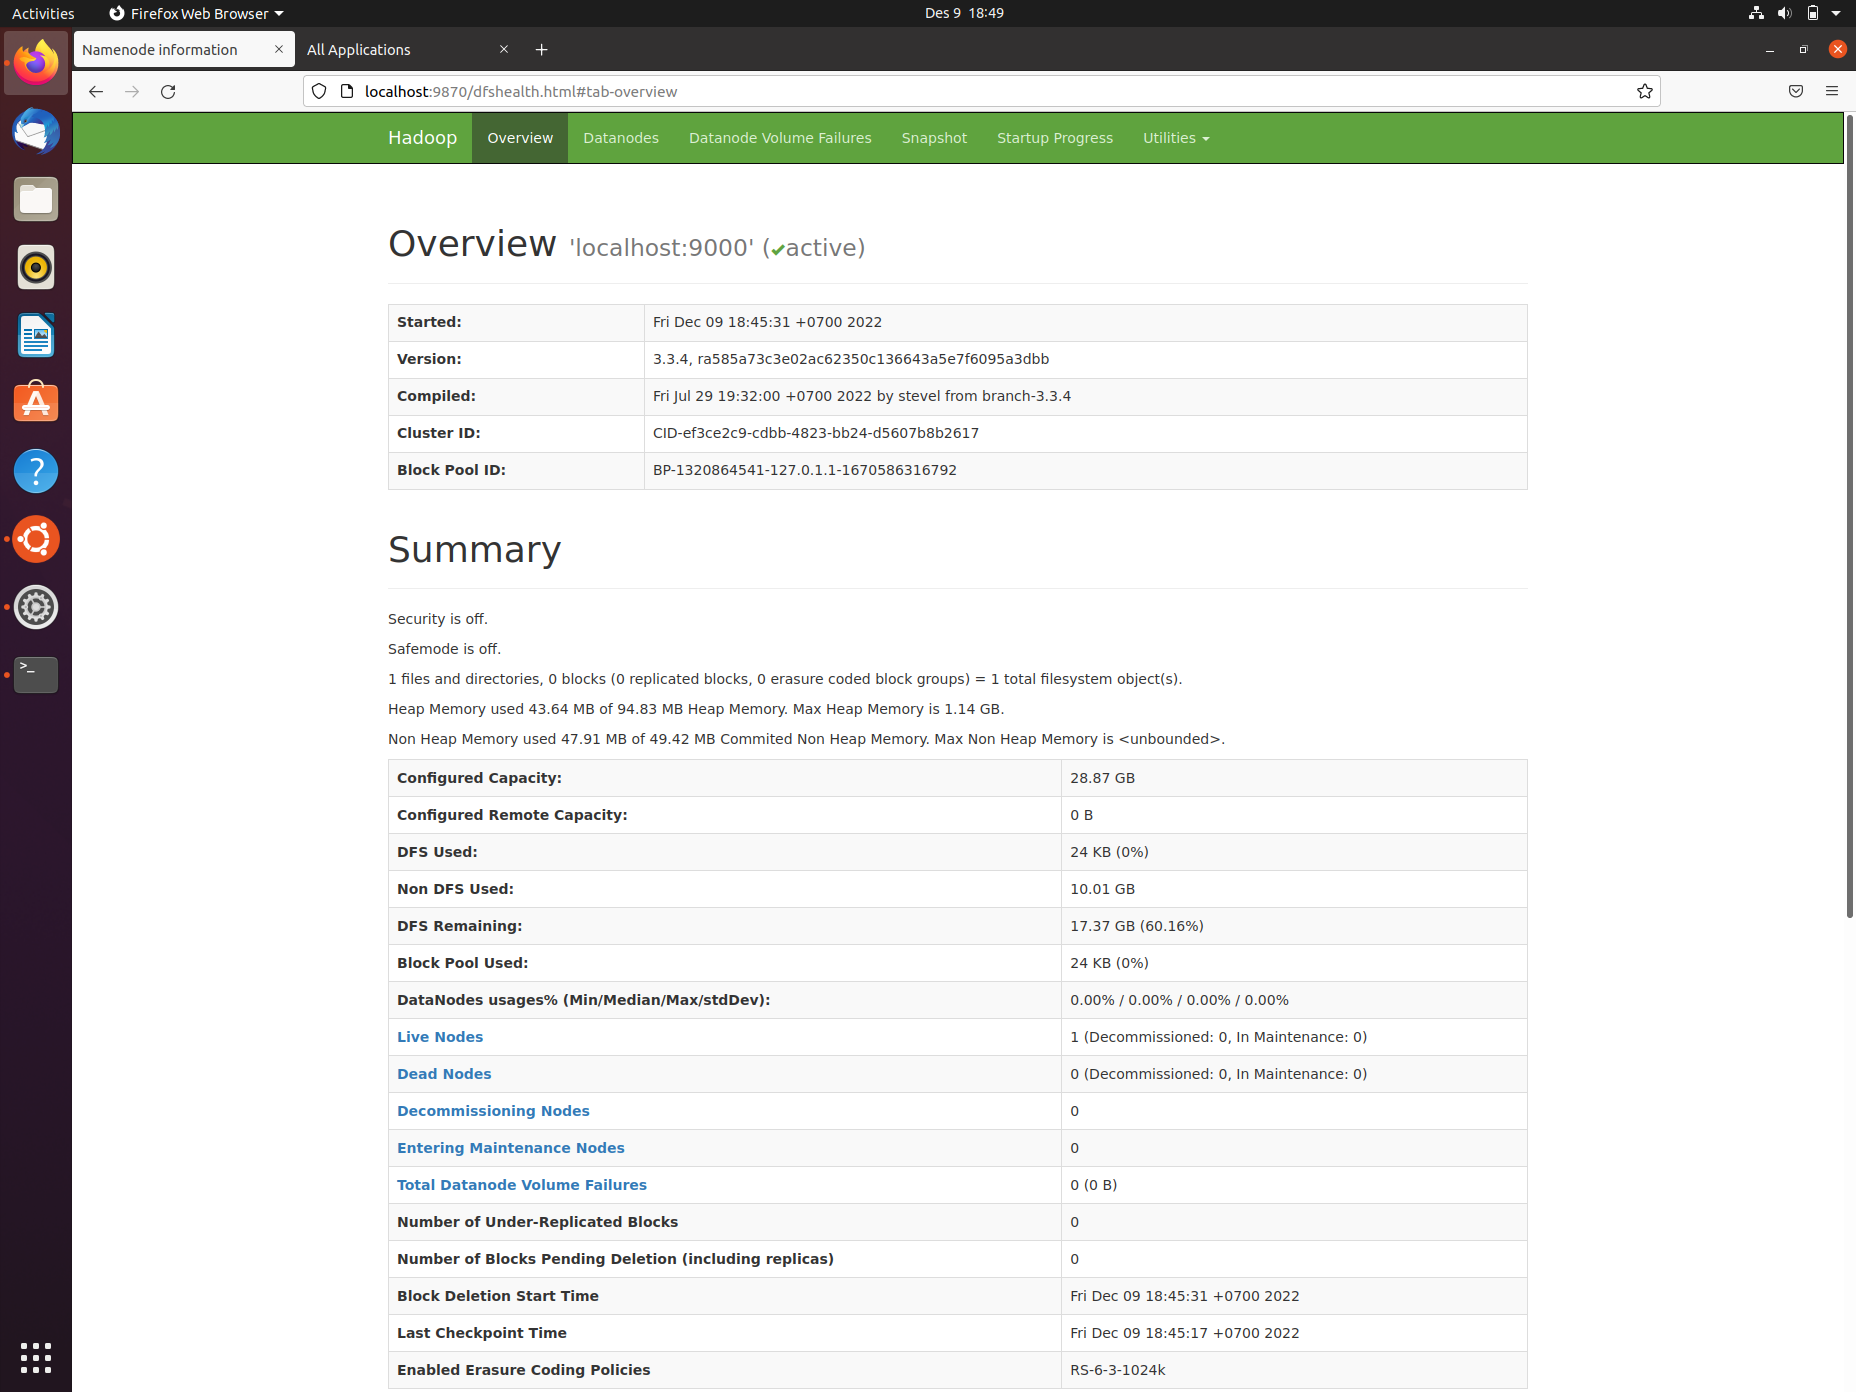
\includegraphics[width=\textwidth]{localhost9870-resha}
\caption{local host 9870 akses}
\label{gam:perkuliahan-22-09}
\end{figure}

\item Kesimpulan
Pada Instalasi Apache Hadoop membutuhkan ruang yang cukup besar untuk mengekstrak file Apache Hadoop. Penginstalaan Apache Hadoop harus dilakukan sesuai step, begitu juga pada saat konfigurasi. Konfigurasi ini bertujuan untuk memudahkan user dalam memonitoring ekosistem di dalam Hadoop. Saat mengkonfigurasi terdapat perintah untuk membuat format HDFS yang berfungsi menyimpan suatu data dengan cara membaginya menjadi potong-potongan data yang disebut blok berukuran 64 MB dan kemudian disimpan pada node-node yang tersebar dalam kluster. Node-node yang ada adalah name node dan data node. Sehingga saat mengecek Hadoop service dengan perintah jps, kedua node tersebut harus tersedia sebagai pendukung saat dilakukan akses web browser dengan local host 9870 dan 8088 berhasil.

\end{enumerate}

\newday{\textbf{24 November 2022}}
\begin{enumerate}
\item Kendala dan Solusi
Pada proses instalasi git dan konfigurasi git dengan github, saya sebagai praktikan tidak mengalami kendala sama sekali.

\item Kesimpulan
Pada instalasi git dan konfigurasi git dengan github bertujuan untuk menjalankan perintah-perintah git melalui penyimpan local dan menyimpan hasil pekerjaan pada github. Penyimpanan pekerjaan dapat dilakukan dengan mudah pada github dengan hanya melakukan git push.

\end{enumerate}

\newday{\textbf{01 Desember 2022}}
\begin{enumerate}
\item Kendala dan Solusi
Pada program WordCount bawaan Hadoop, tidak ada kendala yang saya alami.

\begin{figure}[!ht]
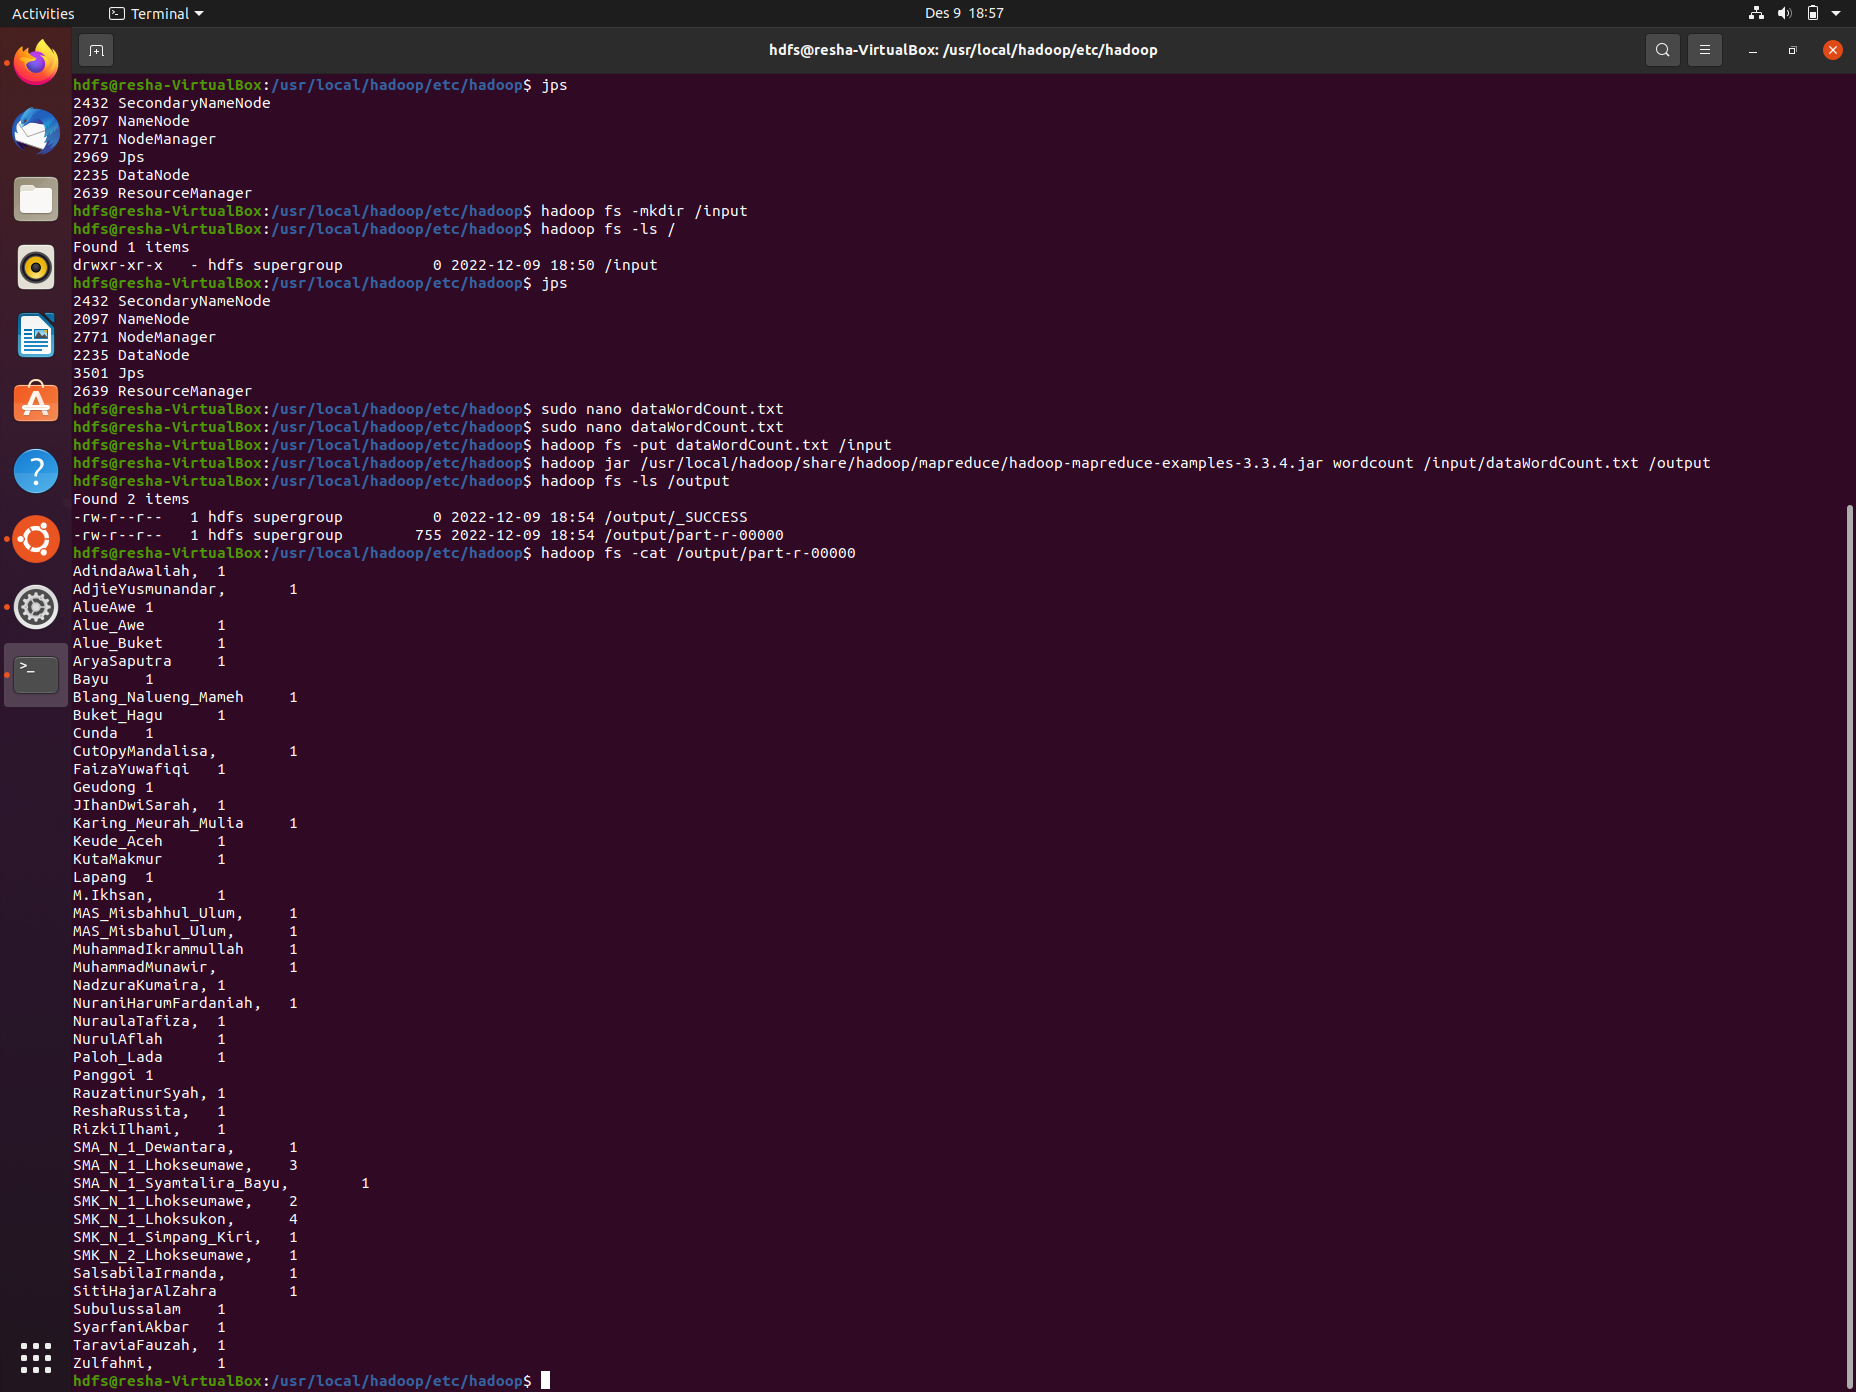
\includegraphics[width=\textwidth]{langkah6dan7-resha}
\caption{Hasil perhitungan dengan WordCount Hadoop berdasarkan data output}
\label{gam:perkuliahan-08-12}
\end{figure}

\item Kesimpulan
Pada Hadoop terdapat program untuk menghitung jumlah kata (WordCount) yang ada pada data. Untuk menghitung jumlah kata, saya sebagai praktikan melakukan input data terlebih dahulu, kemudian memprosesnya, sehingga menghasilkan data output. Data output tersebut yang digunakan untuk Hadoop menjalankan programnya yaitu WordCount.
Data yang saya input disini adalah data mahasiswa (nama, asal sekolah, dan alamat). Saat melihat hasil perhitungan pada data output, akan ditampilkan jumlah kata dari tiap-tiap nama, asal sekolah, dan alamat mahasiswa.

\end{enumerate}

\newday{\textbf{02 Desember 2022}}
\begin{enumerate}
\item Kendala dan Solusi
% jelaskan kendala dan penyebab yang dialami saat mengikuti praktikum serta solusi atau langkah-langkah yang telah dilakukan

\item Kesimpulan
% berikan kesimpulan dari praktikum yang telah dikerjkan

\end{enumerate}

\newday{\textbf{08 Desember 2022}}
\begin{enumerate}
\item Kendala dan Solusi
% jelaskan kendala dan penyebab yang dialami saat mengikuti praktikum serta solusi atau langkah-langkah yang telah dilakukan

\item Kesimpulan
% berikan kesimpulan dari praktikum yang telah dikerjkan

\end{enumerate}

\newday{\textbf{09 Desember 2022}}
\begin{enumerate}
\item Kendala dan Solusi
% jelaskan kendala dan penyebab yang dialami saat mengikuti praktikum serta solusi atau langkah-langkah yang telah dilakukan

\item Kesimpulan
% berikan kesimpulan dari praktikum yang telah dikerjkan

\end{enumerate}
\newthought{\textbf{Rizki Ilhami - 2020903430042 - TRKJ 3B}}

\newday{\textbf{1 Desember 2022}}
\begin{enumerate}
\item Kendala dan Solusi
% jelaskan kendala dan penyebab yang dialami saat mengikuti praktikum serta solusi atau langkah-langkah yang telah dilakukan

\item Kesimpulan
% berikan kesimpulan dari praktikum yang telah dikerjkan

\end{enumerate}

\newday{\textbf{2 Desember 2022}}
\begin{enumerate}
\item Kendala dan Solusi
% jelaskan kendala dan penyebab yang dialami saat mengikuti praktikum serta solusi atau langkah-langkah yang telah dilakukan

\item Kesimpulan
% berikan kesimpulan dari praktikum yang telah dikerjkan

\end{enumerate}
	
\newthought{\textbf{Salsabila Irmanda - 2020903430048 - TRKJ 3B}}
\newday{\textbf{1 Desember 2022}}
\begin{enumerate}
\item Kendala dan Solusi
% jelaskan kendala dan penyebab yang dialami saat mengikuti praktikum serta solusi atau langkah-langkah yang telah dilakukan

\item Kesimpulan
% berikan kesimpulan dari praktikum yang telah dikerjkan

\end{enumerate}


\newthought{\textbf{Adinda Awaliah - 2020903430004 - TRKJ 3B}}

\newday{\textbf{22 September 2022}}
\begin{enumerate}
\item Kendala dan Solusi
% jelaskan kendala dan penyebab yang dialami saat mengikuti praktikum serta solusi atau langkah-langkah yang telah dilakukan

\item Kesimpulan
% berikan kesimpulan dari praktikum yang telah dikerjkan

\end{enumerate}


\newthought{\textbf{Adinda Awaliah - 2020903430004 - TRKJ 3B}}

\newday{\textbf{22 September 2022}}
\begin{enumerate}
\item Kendala dan Solusi
% jelaskan kendala dan penyebab yang dialami saat mengikuti praktikum serta solusi atau langkah-langkah yang telah dilakukan

\item Kesimpulan
% berikan kesimpulan dari praktikum yang telah dikerjkan

\end{enumerate}


\newthought{\textbf{Taravia Fauzah- 2020903430054 - TRKJ 3B}}

\newday{\textbf{13-20 Oktober 2022} - Instalasi dan Konfigurasi Hadoop}
\begin{enumerate}
\item Kendala dan Solusi
% jelaskan kendala dan penyebab yang dialami saat mengikuti praktikum serta solusi atau langkah-langkah yang telah dilakukan
\newline praktikum pertama yaitu instalasi apache hadoop. selama mengerjakan praktikum mengikuti modul tidak ada kendala

\begin{figure}[!ht]
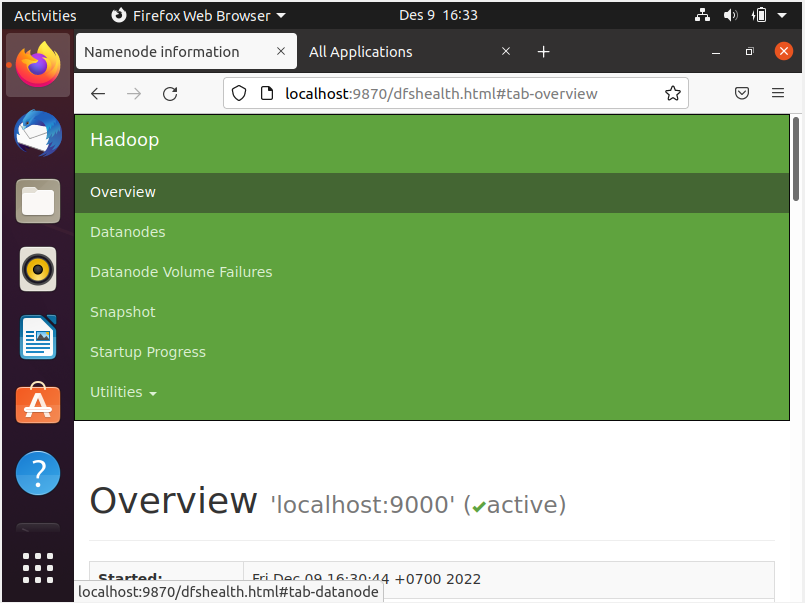
\includegraphics[width=\textwidth]{TaraviaFauzah/akses-localhost-9078}
\caption{hasil dari cek hadoop service}
\label{gam:perkuliahan15-9}
\end{figure}

\begin{figure}[!ht]
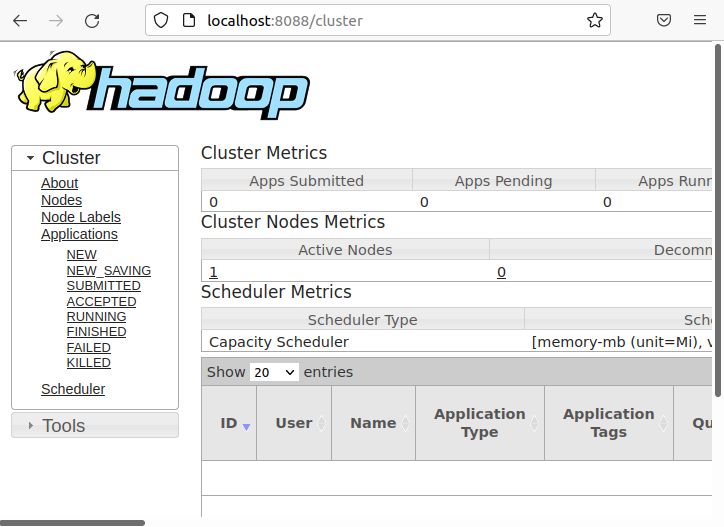
\includegraphics[width=\textwidth]{TaraviaFauzah/akses-localhost-8088}
\caption{hasil dari cek hadoop service}
\label{gam:perkuliahan15-9}
\end{figure}

\item Kesimpulan
% berikan kesimpulan dari praktikum yang telah dikerjkan
\newline Berhasil mendownload dan menginstal Apache hadoop dan sudah bisa di jalankan 
\end{enumerate}

\newday{\textbf{10 November 2022} - WordCount bawaan Hadoop}
\begin{enumerate}
\item Kendala dan Solusi
% jelaskan kendala dan penyebab yang dialami saat mengikuti praktikum serta solusi atau langkah-langkah yang telah dilakukan
\newline pada praktikum kali ini membuat program WordCount Bawaan Hadoop.pada saat praktikum tidak ada kendala hanya saja error karena salah menulis perintah.

\begin{figure}[!ht]
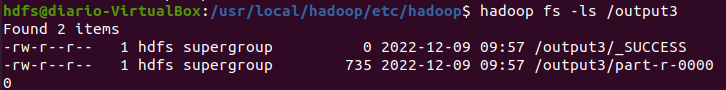
\includegraphics[width=\textwidth]{TaraviaFauzah/output}
\caption{hasil dari hadoop fs}
\label{gam:perkuliahan1-10}
\end{figure}

\begin{figure}[!ht]
\includegraphics[width=\textwidth]{TaraviaFauzah/output1}
\caption{hasil dari hadoop fs}
\label{gam:perkuliahan1-10}
\end{figure}

\begin{figure}[!ht]
\includegraphics[width=\textwidth]{TaraviaFauzah/output1_1}
\caption{hasil dari hadoop fs}
\label{gam:perkuliahan1-10}
\end{figure}

\item Kesimpulan
% berikan kesimpulan dari praktikum yang telah dikerjkan
\newline langkah praktikum ini adalah untuk memahami proses cara kerja pada hadoop dalam memproses data input sehingga menghasikan sebuah output. wordcount adalah program untuk menghitung jumlah kata dalam inpu.

\end{enumerate}

\newday{\textbf{17 November 2022} - WordCount dengan Java}
\begin{enumerate}
\item Kendala dan Solusi
% jelaskan kendala dan penyebab yang dialami saat mengikuti praktikum serta solusi atau langkah-langkah yang telah dilakukan
\newline pada praktikum kali ini membuat program WordCount dengan java.pada saat praktikum memiliki error tapi errornya di sebabkan tidak teliti saat menulis codingan yang ada di modul.solusinya harus lebih teliti saat mengerjakan codingan tersebut.

\begin{figure}[!ht]
\includegraphics[width=\textwidth]{TaraviaFauzah/hasil1}
\caption{hasil dari hadoop fs WordCount}
\label{gam:perkuliahan2-12}
\end{figure}

\begin{figure}[!ht]
\includegraphics[width=\textwidth]{TaraviaFauzah/hasil2}
\caption{hasil dari hadoop fs WordCount}
\label{gam:perkuliahan2-12}
\end{figure}

\begin{figure}[!ht]
\includegraphics[width=\textwidth]{TaraviaFauzah/hasil2_2}
\caption{hasil dari hadoop fs WordCount}
\label{gam:perkuliahan2-12}
\end{figure}

\item Kesimpulan
% berikan kesimpulan dari praktikum yang telah dikerjkan
\newline berhasil menjalan program WordCount dengan java

\end{enumerate}

\newday{\textbf{24 November 2022} - instalasi apache Spark (Pyspark)}
\begin{enumerate}
\item Kendala dan Solusi
% jelaskan kendala dan penyebab yang dialami saat mengikuti praktikum serta solusi atau langkah-langkah yang telah dilakukan
\newline pada praktikum kali ini instalasi apache spark (pyspark)tidak ada kendala.

\begin{figure}[!ht]
\includegraphics[width=\textwidth]{TaraviaFauzah/pyspark version}
\caption{hasil dari pyspark version}
\label{gam:perkuliahan2-15}
\end{figure}

\item Kesimpulan
% berikan kesimpulan dari praktikum yang telah dikerjkan
\newline berhasil menjalan pyspark yang sudah terinstall.
\end{enumerate}

\newday{\textbf{1 Desember 2022} - Program WordCount dengan Python}
\begin{enumerate}
\item Kendala dan Solusi
\newline pada praktikum kali ini membuat program wordcount dengan python,pada saat mengeisi codingan di nanonya harus lebih teliti supaya tidak terjadi error.

\begin{figure}[!ht]
\includegraphics[width=\textwidth]{TaraviaFauzah/hasil WordCountPython2}
\caption{lihat hasil dari WordCountPython }
\label{gam:perkuliahan2-15}
\end{figure}

\begin{figure}[!ht]
\includegraphics[width=\textwidth]{TaraviaFauzah/hasil WordCounPython1}
\caption{Cek hasil dari WordCountPython }
\label{gam:perkuliahan2-15}
\end{figure}

\item Kesimpulan
\newline berhasil membuat pemograman WordCount dengan Python.
\end{enumerate}

\newday{\textbf{8 Desember 2022} - Program WordCount dengan PySpark}
\begin{enumerate}
\item Kendala dan Solusi
\newline pada praktikum kali ini membuat program wordcount dengan pySpark,pada saat mengeisi codingan di nanonya harus lebih teliti supaya tidak terjadi error.

\begin{figure}[!ht]
\includegraphics[width=\textwidth]{TaraviaFauzah/hasil WordCountPySpark1}
\caption{cek hasil dari WordCountPySpark }
\label{gam:perkuliahan2-15}
\end{figure}

\begin{figure}[!ht]
\includegraphics[width=\textwidth]{TaraviaFauzah/hasil WordCountPySpark2}
\caption{lihat hasil dari WordCountPySpark }
\label{gam:perkuliahan2-15}
\end{figure}

\item Kesimpulan
\newline berhasil membuat pemograman WordCount dengan PySpark.
\end{enumerate}


\newthought{\textbf{Zulfahmi - 2020903430056 - TRKJ 3B}}

\newday{\textbf{01 Desember 2022}}
\begin{enumerate}
\item Kendala dan Solusi
% jelaskan kendala dan penyebab yang dialami saat mengikuti praktikum serta solusi atau langkah-langkah yang telah dilakukan

\item Kesimpulan
% berikan kesimpulan dari praktikum yang telah dikerjkan

\end{enumerate}

\newday{\textbf{02 Desember 2022}}
\begin{enumerate}
\item Kendala dan Solusi
% jelaskan kendala dan penyebab yang dialami saat mengikuti praktikum serta solusi atau langkah-langkah yang telah dilakukan

\item Kesimpulan
% berikan kesimpulan dari praktikum yang telah dikerjkan

\end{enumerate}

\newday{\textbf{08 Desember 2022}}
\begin{enumerate}
\item Kendala dan Solusi
% jelaskan kendala dan penyebab yang dialami saat mengikuti praktikum serta solusi atau langkah-langkah yang telah dilakukan

\item Kesimpulan
% berikan kesimpulan dari praktikum yang telah dikerjkan

\end{enumerate}

\clearpage
\bibliographystyle{plain}
\bibliography{lab_notes}

\end{document}

%%%%%%%%%%%%%%%%%%%%%%%%%%%%%%%%%%%%%%%%%%%%%%%%%%%%%%%%
